\chapter{基于内存的分布式键值存储系统}
\label{chapter:sedna}

\section{引言}
云计算平台上的存储系统和传统的网络存储系统不同,它不仅仅要对外服务接受来自客户端的读写请求,更重要的是为云计算平台中运行的分布式任务提供并发的数据读写能力。图\ref{fig:app}展示了一个典型的云计算环境下,数据中心内部存储的架构图:存储通过大量的廉价个人计算机构成,存储系统不仅仅接受来自外界的读写请求,更需要支撑数据中心内部运行的应用程序的读写请求。

\begin{figure}[h!]
\centering
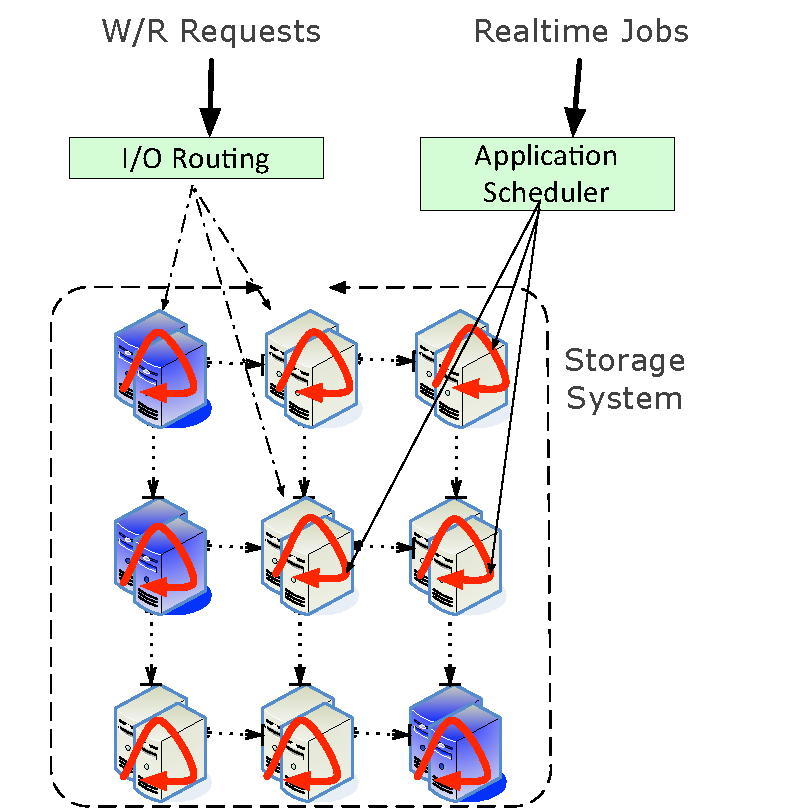
\includegraphics[height=3in, width=3.5in]{../figures/app.pdf}
\caption{典型的云计算环境下数据中心中存储架构图}
\label{fig:app}
\end{figure}

为了存储各种不同类型的数据并支撑不同类型的应用程序,云计算领域出现了多种分布式存储系统。早期以Google File System\cite{Ghemawat2003}为代表的块式存储多用来存储只会被追加写的较大的文件,因此适合连续的对数据块进行读取。这类存储系统最早出现在搜索引擎相关的系统中,主要是由于通用搜索引擎对廉价集群上进行海量数据存储的需求。后来以Dynamo\cite{decandia2007dynamo}为代表的分布式的键值存储系统开始出现。这类存储系统专用于存储较小的数据且支持对这些数据进行随机读写。在键值存储系统的基础上,出现了被称为NoSQL\cite{nosqldatabase}的海量结构化存储系统,如Bigtable\cite{chang2008bigtable}、Cassandra\cite{lakshman2010cassandra}等,这类存储系统多用来存储具有结构化信息的数据,数据按\textit{表}组织,表中每一个单元存储的数据都较小并且支持随机的读写。

这些存储系统虽然在存储的数据类型以及所支撑的应用类型上有区别,但它们都是基于硬盘(Hard Driver)构建的持久分布式存储系统。在对读写性能要求苛刻的场景下,它们的性能是不能接受的。比如Facebook网站的后台数据中心每秒需要承担10亿次随机读\cite{nishtala2013scaling},在这样的负载要求下,数据中心内部需要部署像Redis\cite{redis},Memcached\cite{memcachedproject}这样的分布式内存缓存来提高读写速率。分布式缓存系统通过在内存中构建非持久的哈希表为应用提供高速随机访问能力。不过作为缓存系统,其不能脱离一个持久存储系统独立存在,更无法保证数据的持久性。2009年提出的RamCloud\cite{ousterhout2010case}在完全基于内存的基础上为数据提供了持久性保障以及快速数据恢复能力,可以作为独立的高速分布式存储系统使用。

从分布式存储的发展路径可以看出,随着社交网络,电子商务,在线广告系统的发展,小的、零散的原始数据现在已经成为应用程序最主要的数据来源,云计算环境下的存储系统也在向高速读写、随机访问、海量小数据的方向发展。在本章中,我们将介绍另一个完全基于内存实现的持久化的分布式键值存储系统——Sedna。该系统通过引入新的集群架构、节点管理算法、以及新的API进一步提高了海量内存存储系统的存储容量、随机访问速度、数据一致性等方面的性能,并通过为用户提供了一个简单、有效的实时API来支持各类实时应用。\ref{section:relevant}节介绍现有存储系统上的相关工作,以及内存存储的合理性和主要挑战。\ref{section:techs}节详细描述Sedna的架构和实现细节,\ref{section:exp3}节通过实验着重分析了Sedna的读写性能,\ref{section:con3}节对本章进行了小结。

\section{相关工作简介}
\label{section:relevant}

\subsection{相关分布式存储系统介绍}
Google File System由Google公司与2003年提出的使用海量廉价个人计算机实现的基于块的大规模分布式文件系统,其基本架构如图\ref{fig:gfsarch}所示,包括一个master和多个chunkserver组成。文件系统的层次结构和名字空间都存放在GFS Master节点中,客户端应用程序首先通过查询GFS master来获得欲访问的文件所在节点信息(chunk location),然后通过向特定的节点发送读写请求来完成数据传输过程。

\begin{figure}[h!]
\centering
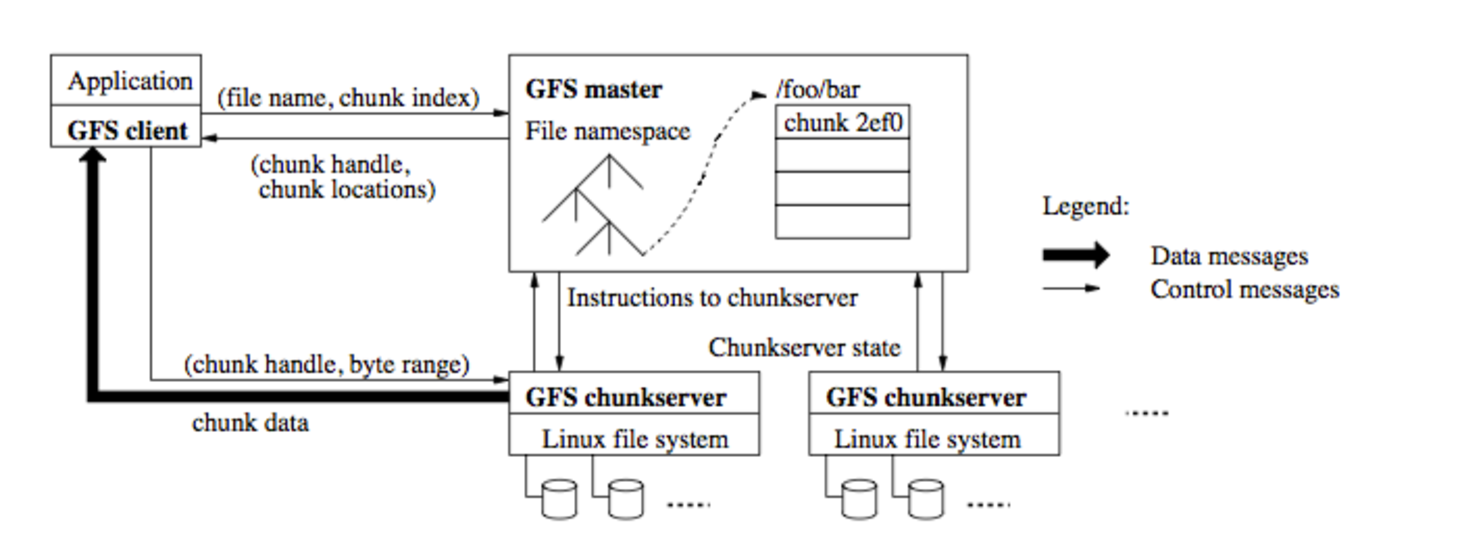
\includegraphics[width=6in]{../figures/gfsarch.pdf}
\caption{GFS文件系统的架构}
\label{fig:gfsarch}
\end{figure}

Hadoop Distributed File System(HDFS)是Apach基金会基于GFS实现的一套开源分布式存储系统。如图\ref{fig:hdfsarch}所示,HDFS中NameNode和DataNode分别对应了GFS中的Master和Chunkserver。类似GFS,任何一个文件都由预定义大小(默认64MB)的块组成,这些块被冗余存储于多个DataNode上(默认情况下,每一个块会存储在三个节点中)。由于HDFS运行在由海量个人计算机构成的数据中心中,节点失效和网络故障比较常见,通过多备份实现了系统的可用性和容错性。每一个DataNode需要和NameNode维持一个周期心跳用来检测节点是否失效以及网络是否可用,当NameNode发现某节点失效的时候会利用备份节点的数据来提供服务,并且尝试恢复失效节点,以维持每一个数据块多备份的状态。由于每一个客户端在访问HDFS中的数据时都需要向NameNode查询相关数据所在的DataNode位置信息,为了保证多个客户端程序读写的性能,HDFS的实现中会将所有的命名空间信息都存放在NameNode的内存中。

\begin{figure}[h!]
	\centering
	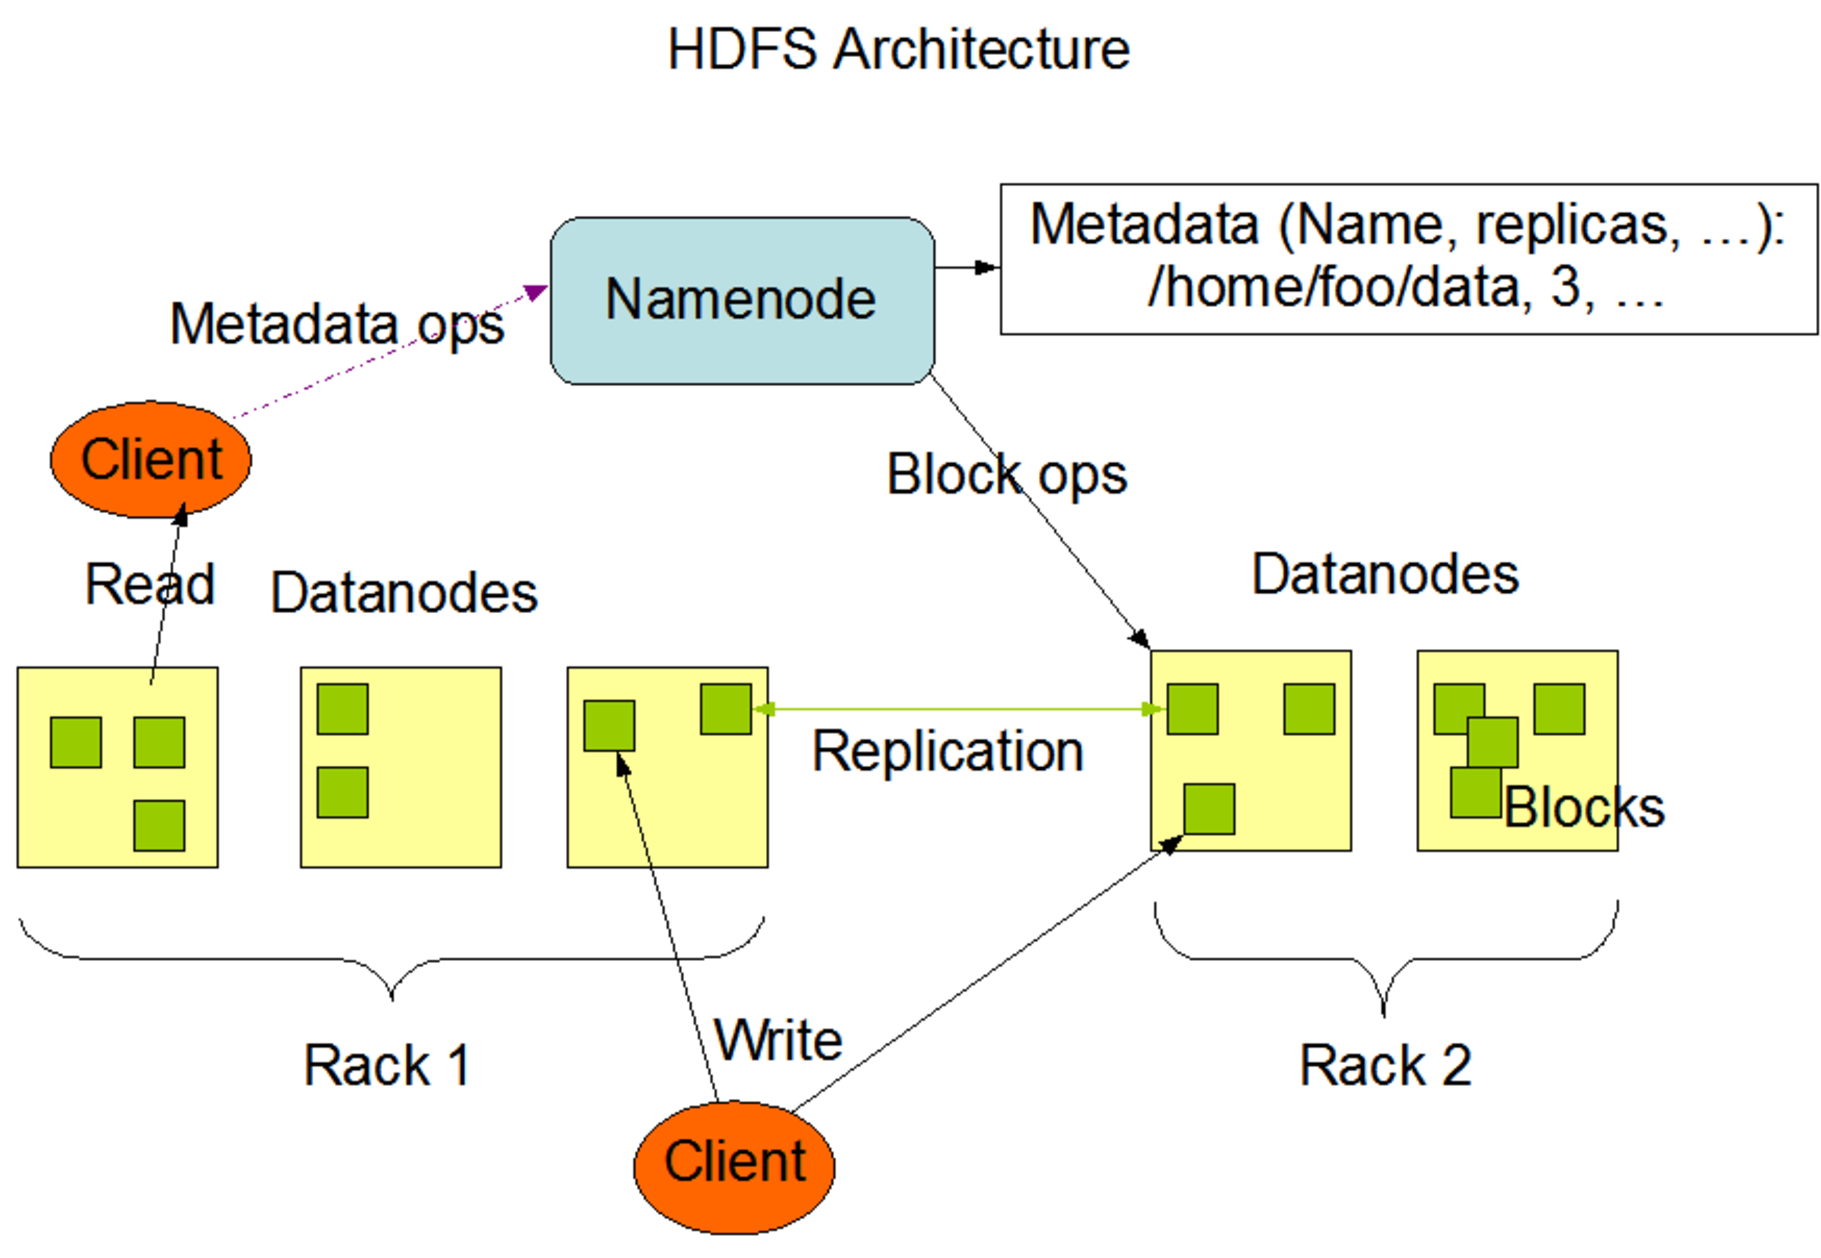
\includegraphics[width=5in]{hdfsarchitecture.pdf}
	\caption{HDFS文件系统架构图}
	\label{fig:hdfsarch}
\end{figure}

HDFS这种以数据块为基本单元的方法提高了系统对于海量文件的存储能力。通过单个NameNode可以管理成千上万服务器构成的存储集群。但是这种方案同时也带来了一些很明显的问题,其中两个比较典型的是:NameNode的单点故障和集群存储容量受限于单台服务器性能。

对于单点故障问题,2011年Borthakur\cite{borthakur2011apache}提出了使用AvatarNode代替NameNode和SecondaryNameNode的方案,系统架构如图(\ref{fig:avatar})所示:HDFS集群包含两个avatar节点,active avatar和standby avatar。任一个avatar节点实际上都是一个正常的NameNode的包裹。HDFS文件系统镜像和日志都存放在NFS中,而不是本地。活动的avatar节点将所有的事务写入在NFS中的log文件中,与此同时,standby avatar节点将从NFS中打开相同的log文件,读入并且不断的将新写入的事务应用到本地存储的命名空间中,从而使得本地的命名空间和当前活跃avatar节点上的命名空间保持尽量一致。所有的DataNode不仅仅和active avatar节点交流还会和standby avatar节点交流,这样就使得standby的avatar节点时刻保持着最新的块位置信息。在active avatar失效的时候,standby avatar节点能够在一分钟内开始提供服务。

\begin{figure}[h!]
\centering
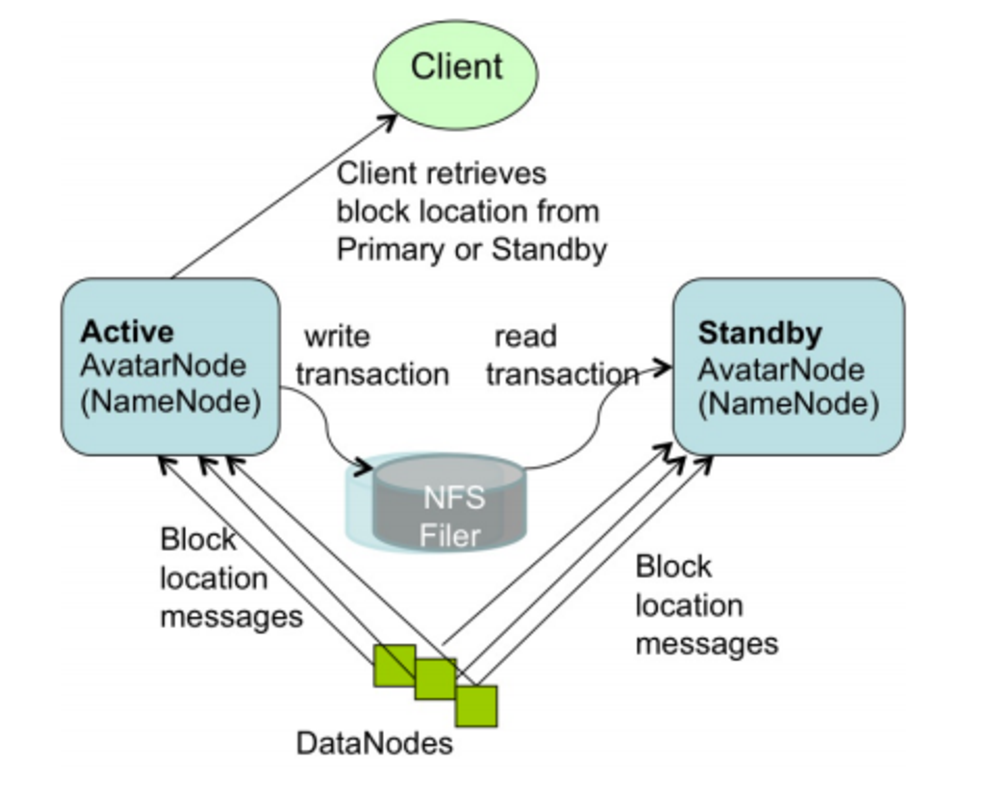
\includegraphics[height=3.5in]{../figures/avatarfb.pdf}
\caption{Avatar Node架构}
\label{fig:avatar}
\end{figure}

容量瓶颈问题同样严重,Konstantin V. Shavachko的论文\cite{shvachko2011apache}详细探讨了HDFS文件系统的瓶颈。通过对当时最大的HDFS集群的实际运行数据的搜集和分析,得到了单个NameNode服务器上内存容量和整个HDFS集群存储容量上限的关系:假设每一个块的位置信息都需要在NameNode中占据超过200个字节的内存,而在一个文件平均包括1.5个块的集群中,每一个文件就大概需要600个字节的内存空间。这样,如果要存储超过1亿个文件,那么NameNode至少就要有60GB的内存。如果该HDFS集群中每一个块为128MB,并且备份三分,那么总的存储空间就是60PB(NameNode需要60GB内存),这也就意味着HDFS的架构不具备线性扩展性。论文\cite{mckusick2009gfs}提出了一种新的GFS Namespace 服务器的架构。这种新的架构包含了数以百计的Namespace服务器,每一个服务器上最多支持超过1亿个文件。由于NameNode容量的提高,每一个文件可以被划分为更加细粒度的块(由64MB可以减少到1MB),用以支持小数据存储。

由于块式存储系统在随机读写上性能较差,出现了多种针对小数据随机访问模式的键值存储系统。Dynamo\cite{decandia2007dynamo}是2006年Amazon公司提出的一种高可用的键值存储系统。从存储内容来说,Dynamo是一种存储键值对的存储系统;从应用场景来说,Dynamo主要应用于\textit{永远可写}的场景中。比如在Amazon网站的购物车应用中,用户任意一次的\textit{加入购物车}动作都应该成功,不管这次请求时数据中心内部是否发生了错误。从架构上来说,Dynamo彻底抛弃了GFS的单中心节点架构,提出了一套基于对等网络的P2P架构。所有的节点都等价的提供服务,节点和节点之间松耦合,单个节点失效不会影响到别的节点。为了提供高可用,高速随机写的能力,Dynamo整合了一系列分布式系统技术:采用动态哈希表和一致性哈希来进行数据划分和复制备份;使用多版本和矢量时钟技术来提供一致性;多副本之间的一致性由仲裁算法来保持一致性;采用反熵(anti-entropy based recovery)的恢复策略;采用基于gossip的分布式故障检测及token协议等。

Megastore\cite{baker2011megastore}是由Google于2011年公开的跨数据中心存储系统。它在保证扩放性的前提下,提供了传统RDBMS具备的易用性,包括强一致性保证、高可用性,并且在细粒度的数据分片中提供了ACID的语义。Megastore通过允许应用程序细粒度的管理数据分片和本地性,从而避免了CAP\cite{gilbert2002brewer}的限制。在Megastore中以EntityGroup作为基本的独立数据集合,一个EntityGroup中的数据并且会在不同的数据中心间同步复制。除此之外,Megastore还使用Paxos\cite{lamport2001paxos}协议避免了之前所提到的分布式主节点需要将写前日志(write-ahead-log)复制到多个节点的耗时操作。

\begin{figure}[h!]
\centering
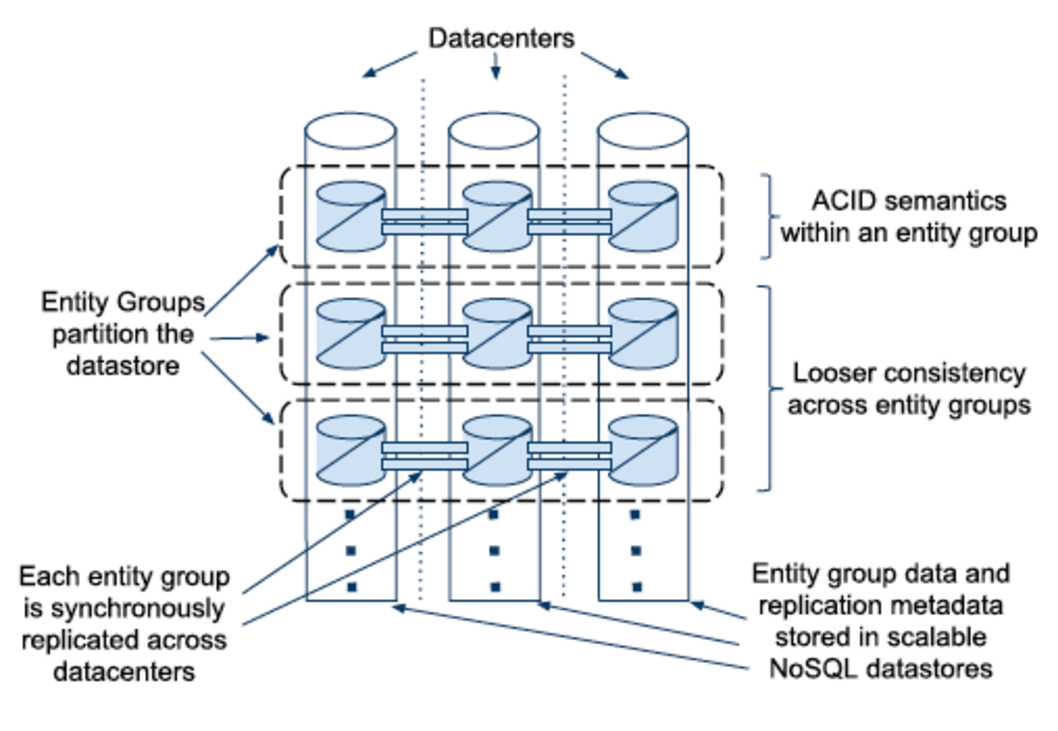
\includegraphics[width=4in]{../figures/megastore.pdf}
\caption{Megastore架构图}
\label{fig:megastore}
\end{figure}

图(\ref{fig:megastore})展示了EntityGroup的结构以及它们是如何在不同的数据中心之间进行复制的。在一个EntityGroup内部的所有操作都依赖于Paxos算法来确保其ACID的语义,而跨EntityGroup的操作则依赖于比较笨重的两阶段提交协议。在一个数据中心内部,Megastore使用Bigtable来做基础的容错存储。Megastore的创新点主要体现在下面几个方面:1)设计了EntityGroup方案给应用程序提供了足够的灵活性;2)使用Paxos算法来保证EntityGroup内部数据的强一致性。3)将分布式存储系统Bigtable和传统SQL模型相结合。

\subsection{内存存储的可行性和相关系统介绍}
实时应用在大规模数据处理应用中比重越来越大,得益于半导体技术的发展使得数
据产生的速度越来越高,数据存储的成本越来越低。实时应用对数据实时性的敏感度较高,
需要存储系统能够提供更高的读写速度。传统的基于磁盘的存储系统在随机读写上的局限性越来越明显。因此在实际应用中,多使用内存缓存系统在磁盘存储系统之上提供高速随机读写的能
力。比如世界上最大的社交网络Facebook,大量使用Memcached作内存缓存。以2009年8月的数据来看\cite{ousterhout2010case},大约其所有在线数据的25\%是保存在Memcached集群的内存中的,缓存提供了96.5\%的平均命中率。如果再算上数据库服务器的内存缓存,那么整个数据集(除去图片)大约有75\%的数据是存放在内存中的。从Facebook数据在内存缓存的比率来看,海量数据的场景下,使用内存来作为唯一的在线存储是可能的。

使用内存缓存系统似乎能够在较高的命中率的基础上以较少的内存代价(如在Facebook中,25\%的数据存储在内存中提供了96.5\%的命中率)来提供较高的平均访问时间。然而,由于磁盘和内存之间处理时间之间差超过1000倍,使得一次未命中会导致非常明显的访问延迟,这往往是不可以接受的。而且缓存机制带来的冷启动、数据抖动都埋下了性能急剧降低的隐患。

\begin{figure}[h!]
  \centering
  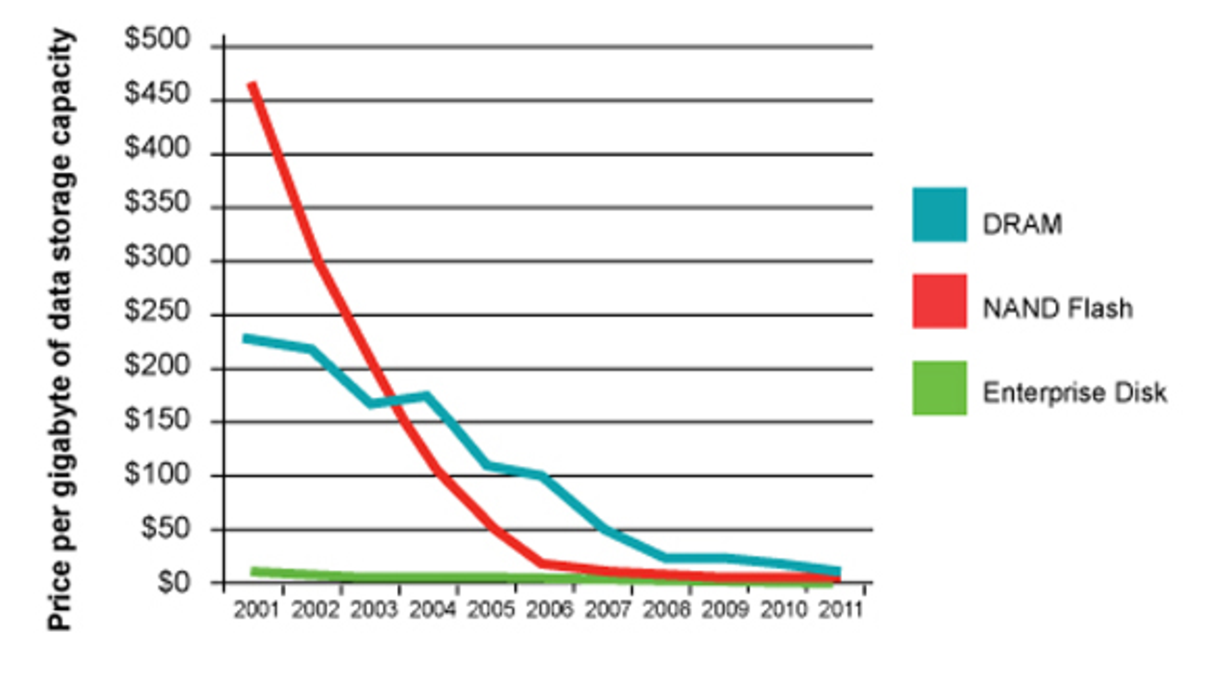
\includegraphics[width=3.5in]{../figures/mp.pdf}
  \caption{最近十年(2001-2011)内存,磁盘,Flash单位Gb的价格趋势分析。}
  \label{fig:price}
\end{figure}

因此在数据中心内部完全使用内存作为主要的存储介质,将硬盘(Hard Disk)作
为备份存储介质逐渐成为提高存储系统性能的主要手段。使用内存作为海量存
储的主要介质的可能性随着内存价格的逐步降低已经越来越大,图
\ref{fig:price}展示了十年来存储每Gb的数据,需要的成本对比图,从图中
我们可以看出来,随着半导体技术的发展,DRAM的成本有了一个极为明显的下降
过程,按照这个趋势,单位GB内存价格将持续走低,未来单机大规模内存会成为
主流。结合表\ref{table:price2}除去数据中心中网络和机架
成本,仅仅计算DRAM的成本,到2020年,我们可以通过假设4,000台服务器的集
群来提供超过1PB内存数据存储能力,而每GB的存储成本只有\$6。


\begin{table}[]\small
\caption{2012年完全使用内存构造海量存储的成本以及2020年的预估\cite{ousterhout2010case}}
\label{table:price2}
\centering
\begin{tabular}{|p{108pt}|c|c|}
\hline
\textbf{} & \textbf{2010} & \textbf{2020}\\
\hline
\textit{服务器数目}& 2,000 & 4,000\\
\hline
\textit{单服务器容量}  & 24GB & 256GB\\
\hline
\textit{总存储容量} & 48TB & 1PB\\
\hline
 \textit{总体成本} & \$3.1M & \$6M \\
 \hline
\textit{每GB成本} & \$65 & \$6 \\
\hline
\textit{每秒操作数} & 2*$10^9$ & 4*$10^9$\\
\hline
\end{tabular}
\end{table}

图\ref{fig:ramcloud}展示了基于内存的RamCloud机群的结构。一个RamCloud实例包括大量存储服务器,每一台存储服务器包含两个部分:1)主(Master)服务负责在内存中管理RAMCloud对象,并且负责处理客户端的请求;2)备份(Backup)服务存储了来自主节点的备份数据,并且将其存放到磁盘和Flash中。每一个RAMCloud实例同时包括一个协作者(Coordinator)服务器,负责管理配置信息,比如存储服务器的网络地址,以及存储对象的位置信息。协作者将对象放置到不同的存储服务器。RamCloud是一个键值存储系统,数据按照键来分布到不同的服务器存储。一个连续的键值组织成一个表,数据量较小的表会存放在一个存储节点中,较大的表会被分割并且存储与多个节点。客户端程序不会控制表的配置,协作者负责存储表和存储服务器之间的映射信息,RAMCloud客户端库将会保存一些缓存信息以减少对协作者的访问。

\begin{figure}[htbp]
	\centering
	\subfloat[RamCloud架构图]{
		\label{fig:ramcloud}
		\begin{minipage}[t]{0.5\textwidth}
			\centering
			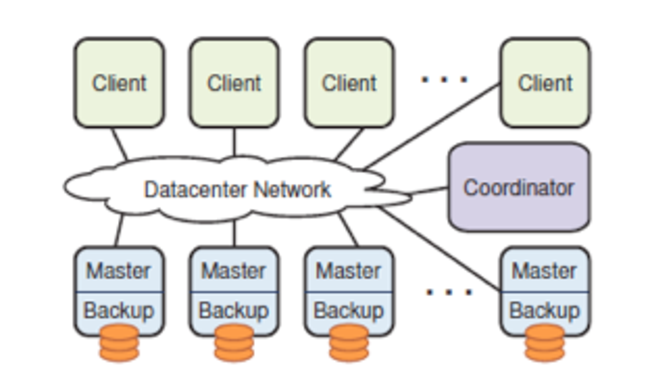
\includegraphics[width=2.8in]{ramcloud.pdf}
		\end{minipage}
	}
	\subfloat[RamCloud Log访问的结构图]{
		\label{fig:ramcloudlog}
		\begin{minipage}[t]{0.5\textwidth}
			\centering
			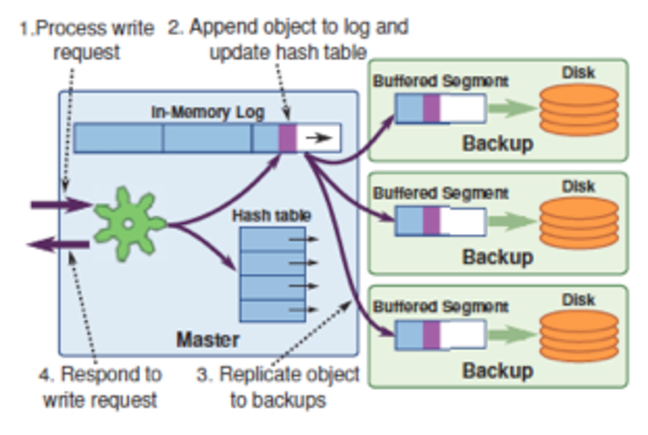
\includegraphics[width=2.8in]{ramcloudlog.pdf}
		\end{minipage}
	}
	\caption{RamCloud系统图示}
\end{figure}

RamCloud通过写备份的方式来保证数据的持久性\cite{ongaro2011fast},如图\ref{fig:ramcloudlog}所示,当一个存储节点中的主服务收到一个写请求的时候,它将首先更新自己内存中的哈希表,并将新的数据转发到多个备份节点中。备份节点将数据缓存在它们的内存中,最终写入本地磁盘。备份节点必须使用备份电源来确保即便在断电时,缓存中的数据也能被写入到本地磁盘中。基于内存在随机访问上的优势,RAMCloud能够极大的降低系统的访问延时,提高吞吐量,非常适应实时应用对存储系统的要求。

\subsection{前人工作的不足}
磁盘作为持久存储介质能够保证服务器在断电或重启后数据不会丢失,内存作为易失性介质,在掉电后所有的数据都会消失。因此基于内存的存储系统第一要解决的问题就是如何持久存储数据。这个问题上,RamCloud提出了一个有效的策略,它将内存中的数据备份到别的节点的内存和磁盘中,并且设计了一套快速恢复的策略,使得数据丢失后能够在几秒的时间内完全恢复。除了数据的持久性问题之外,我们认为还存在几个重要的基础性问题需要解决:
\begin{enumerate}
  \item 扩放性问题。由于单机内存的存储容量远远小于磁盘,内存集群若
    要达到和磁盘集群同样的存储能力需要更多服务器。因此,分布式内存存储
    系统需要具有更好的扩放性。单点故障和单点存储容量瓶颈都是不可以接受的。
    
  \item 读写效率问题。之所以使用内存作为存储介质是希望获得更好的数据
    访问效率从而满足实时应用的需求。传统的数据访问接口对于实时数据改
    变不够敏感,因此我们需要一个对数据改变响应更快的数据访问能力。
\end{enumerate}

\section{基于内存的分布式键值存储系统}
\label{section:techs}
面向实时应用的分布式存储系统应当具备的特点:
\begin{enumerate}
  \item 能够存储海量的小数据。小的、零散的原始数据现在已经成为云计
    算下应用程序最主要的数据来源。比如Twitter这个流行的微型博客系统,
    主要存储的就是不超过140个字符的短消息,在Twitter当前规模下,每
    天都会有超过4亿用户从世界各地提交超过超过三千五百亿条短消息。因此
    一个实时存储系统应该有能力存储下如此多的小数据。
  \item 高速写入速率。依然以Twitter来举例,其每天数以千亿
    计的新消息需要存储,除此之外还包括海量的用户交互信息,要保存并且处理这些不断产生的数据需要非常高的写入效率。
  \item 高速随机读速率。任何时候新的数据写入到存储系统的时候,我们需
    要马上对它们进行处理,这样才能满足实时应用的要求。
  \item 能够帮助开发人员实现实时应用。典型的实时应用需要对用户动作快速产生响应。这一般包括了一系列复杂的分布式计算过程,因此我们希望存储系统能够为编写这样的应用提供更加简洁的接口。
\end{enumerate}

为了应对上面所提出的对存储系统的要求,我们设计并实现了Sedna。相比较传统的基于磁盘的文件系统,Sedna能够提供更快的数据存储和访问速率;相比较现有的内存系统,Sedna在保证数据的持久的基础上,提供了更好的扩放性,并且通过引入触发器的机制为用户提供了更加简单的编写实时应用的数据访问接口。

一个分布式存储系统至少应当包括几个部分:1)元数据管理模块,负责管理所有数据的位置信息、访问历史信息等;2)数据持久化模块,负责保证数据持久存储到磁盘中;3)数据备份恢复模块,负责确保集群中部分节点失效时,数据能够安全恢复;4)节点管理模块,负责自动感知节点的加入和退出动作并进行管理;5)对外的数据访问接口。除此之外,一个完整的生产环境下的存储系统还应当具备状态检测、数据均衡、错误检测、错误恢复、并发管理等等模块。Sedna作为一个原型系统,我们将主要描述其核心的概念和设计,包括:元数据管理模块即数据分割策略、数据备份恢复模块、集群节点管理模块、数据持久化策略以及数据访问接口的设计和实现。在Sedna在很多实现模块上依赖ZooKeeper服务,因此我们在本章中也会单独介绍ZooKeeper的相关实现细节。

表\ref{table:sednatech}展示了Sedna中使用的一些核心的技术及其优点,在后面的几节中将详述它们。


\begin{table}[h!]\small
\caption{Sedna存储系统使用的主要技术列表}
\label{table:sednatech}
\centering
\begin{tabular}{|c|c|c|}
\hline
\textbf{问题} & \textbf{Sedna的解决方案} & \textbf{优点}\\
\hline
数据分割& 带虚节点的一致性哈希 & 更好的扩放性\\
\hline
备份 & 最终一致 & 更高的读写速率\\
\hline
节点管理  & ZooKeeper子集群管理 & 无单点故障\\
\hline
 读写 & 读触发器 & 使用推送提高数据处理速度 \\
 \hline
 容错和错误处理& 心跳协议和读恢复策略 & 较低的错误发现时间\\
\hline
 数据持久化策略& 周期Flush或RamCloud方案 & 提供灵活的持久化方案\\
\hline
\end{tabular}
\end{table}

\subsection{Sedna总体架构}

图\ref{fig:sedna}展示了Sedna存储系统的总体架构图。客户端应用以及集群内部应用都会对Sedna产生请求。外部客户端请求通过请求路由进行负载均衡,内部请求则直接由应用所在节点处理请求。请求的处理过程牵涉到Sedna中两类不同的节点。位于上层的子机群服务器(ZooKeeper Cluster),它们运行着子集群管理服务;以及位于下层的数据节点,它们负责在内存中存储数据。

\begin{figure}[h!]
\centering
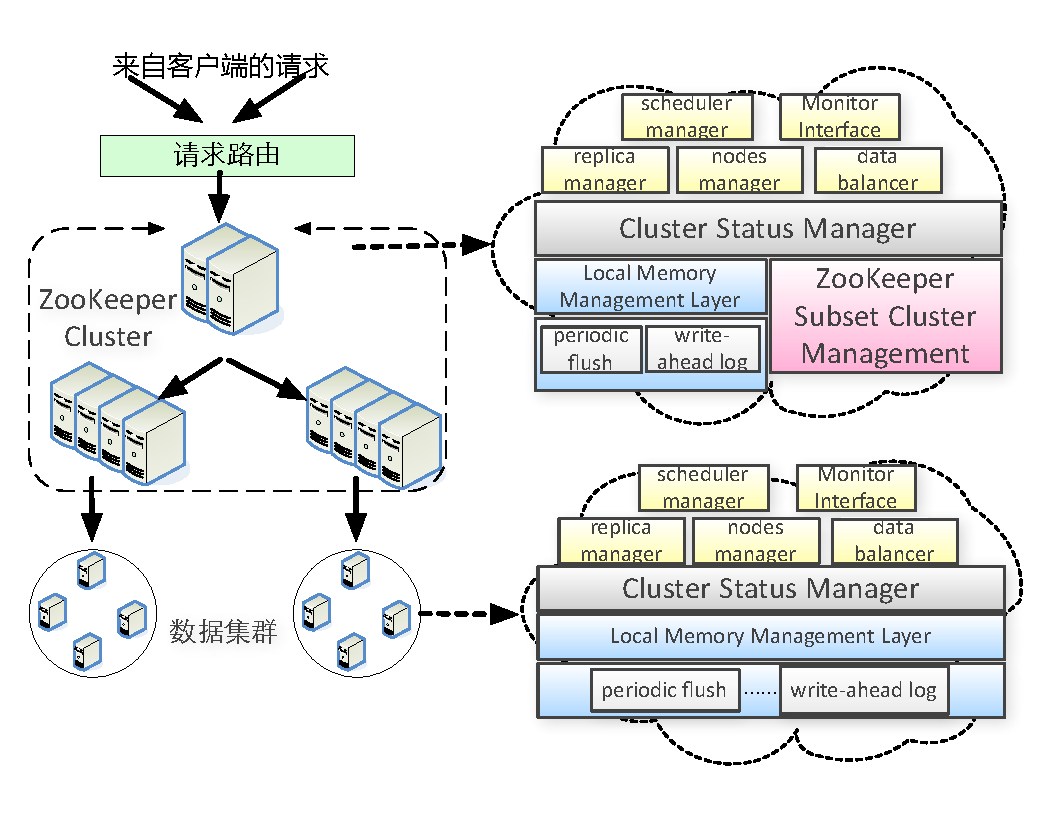
\includegraphics[width=4.5in]{../figures/logic-structure2.pdf}
\caption{Sedna机群的总体架构}
\label{fig:sedna}
\end{figure}

如图\ref{fig:sedna1},一台服务器上运行的一个完整的Sedna实例可以从逻辑上被分为本地部分(local memory store)和分布式组件(Sedna service)部分。本地部分包括本内内存管理层以及持久化存储层,分布式部分则包括了基于ZooKeeper机群一致性信息管理组件。图\ref{fig:sedna}中右侧图中,最上面的层次放置了不同的可插入组件,用来实现Sedna的可扩展的功能,比如接入不同的备份管理策略,或者接入不同的数据同步策略。

\begin{figure}[h!]
\centering
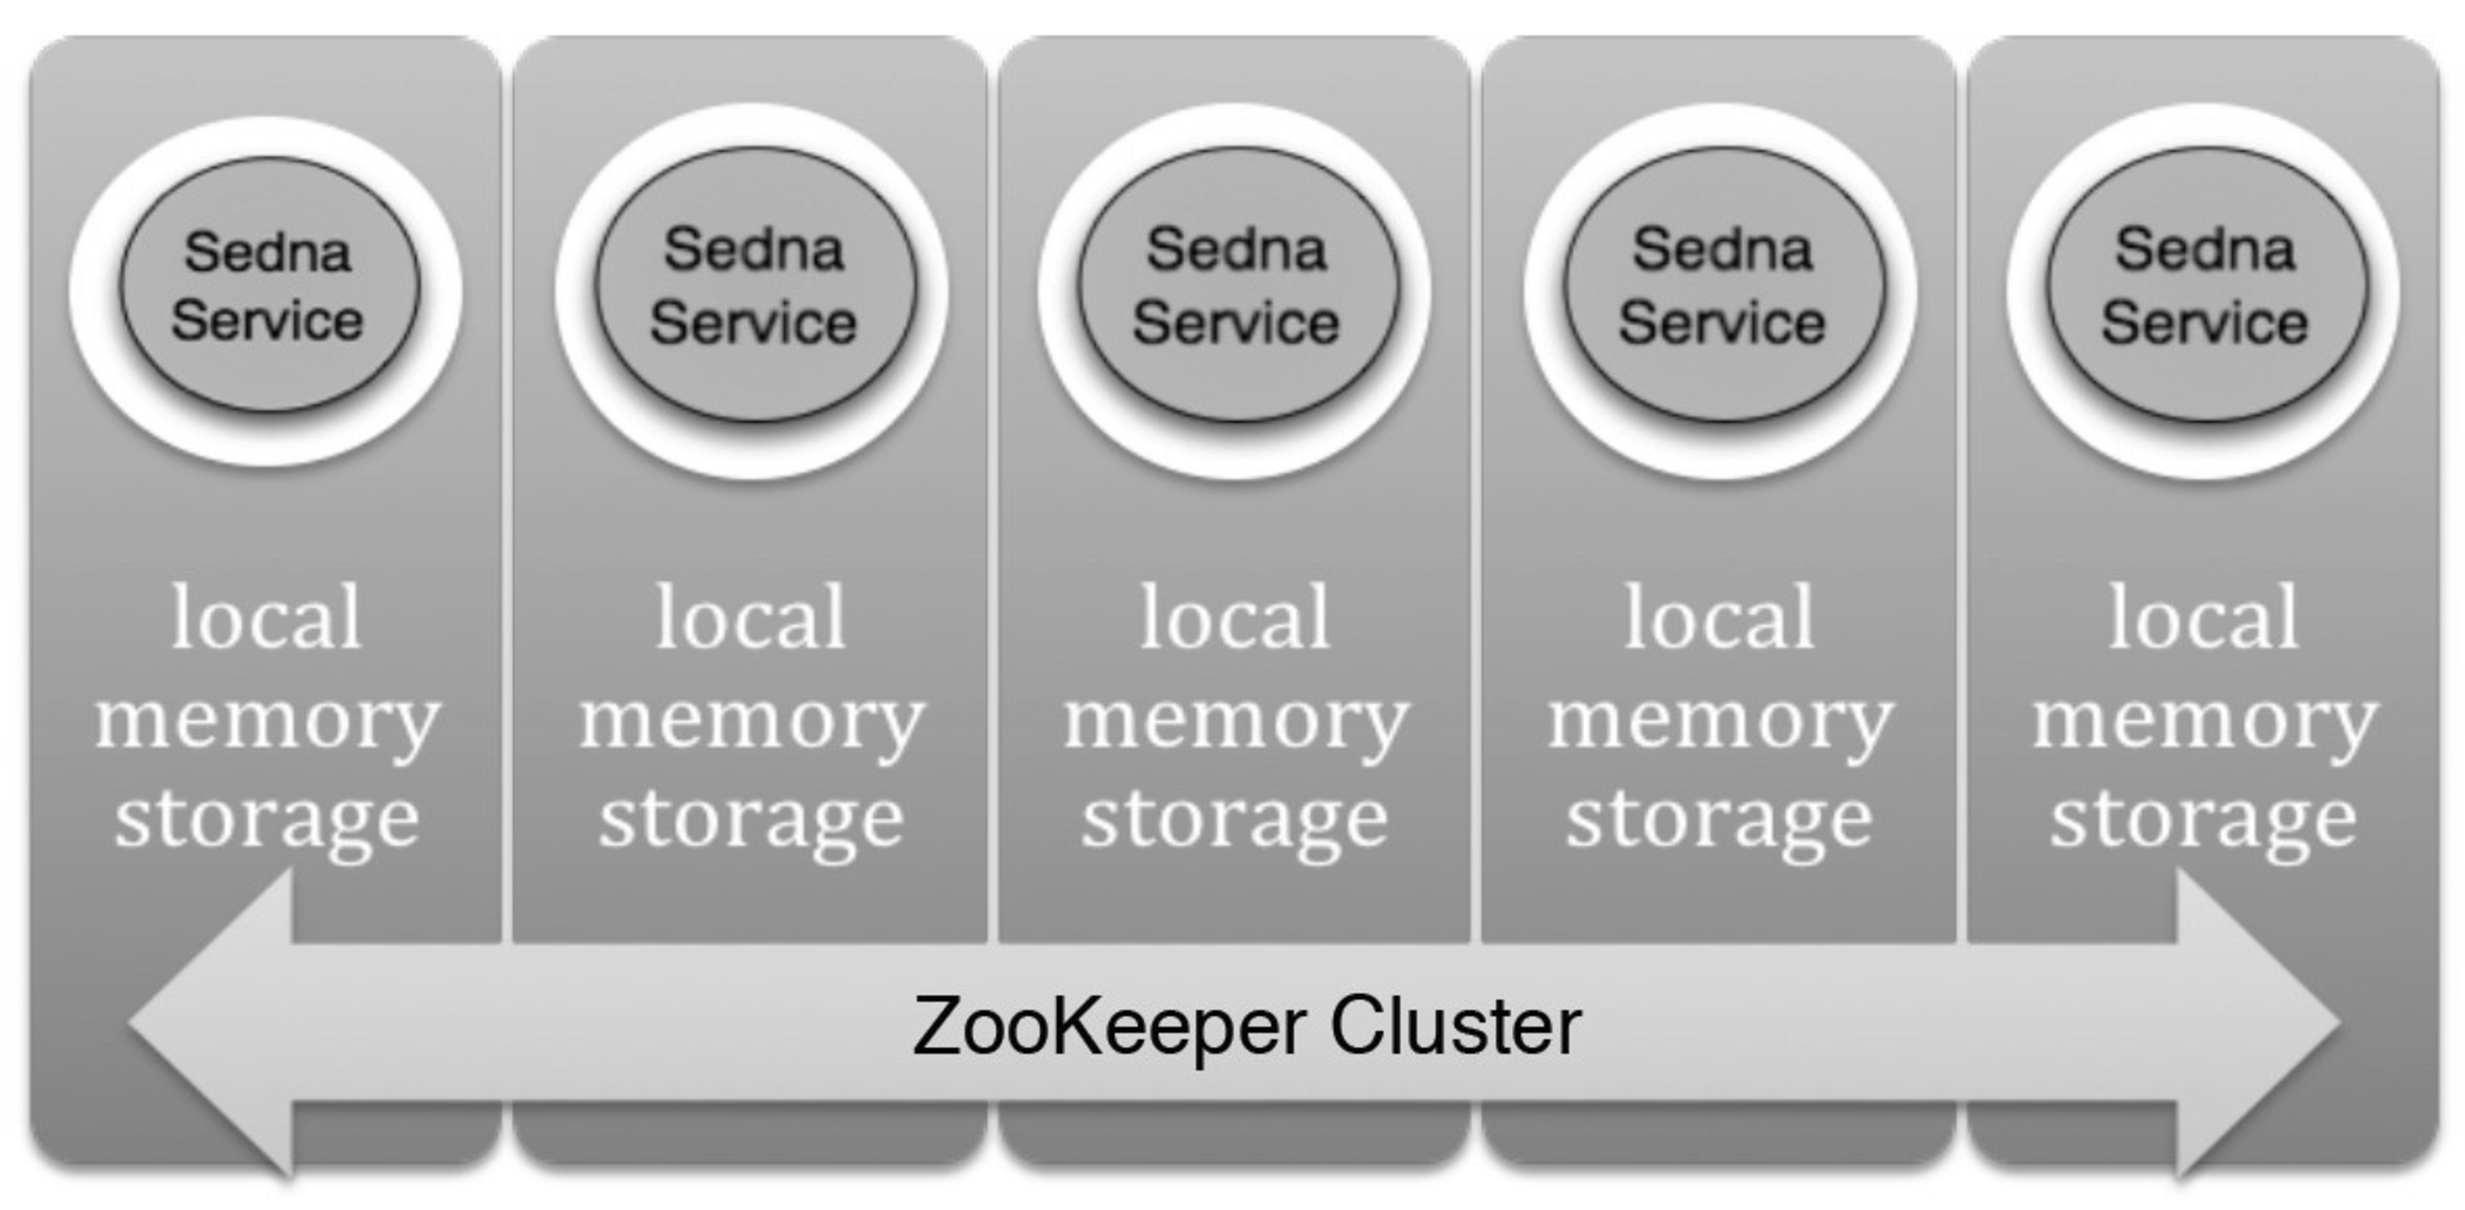
\includegraphics[width=3.5in]{../figures/SednaArc1.pdf}
\caption{每台Sedna服务器内部逻辑结构}
\label{fig:sedna1}
\end{figure}

ZooKeeper子集群是一个运行了ZooKeeper服务的集群,该集群中每一台服务器都选自Sedna集群。该子集群为Sedna提供了强一致性的分布式服务,后面我们会更详细的介绍ZooKeeper以及其在Sedna中实现的优化。总体来说,Sedna需要在下面功能处使用ZooKeeper提供的服务:
\begin{enumerate}
  \item Sedna集群在首次冷启动的时候,使用ZooKeeper的锁服务来选举一个主节
    点进行所有的初始化工作。
  \item 保存Sedna中所有虚节点和物理节点之间的对应关系。每一个物理节点都会在ZooKeeper中新建一个\textit{znode},并且将其所存储的虚节点信息写入该\textit{znode}。
  \item Sedna中物理节点的心跳信息通过ZooKeeper来维护。所有节点上的Sedna实例在初始化时都会向ZooKeeper注册一个临时\textit{znode}节点,并且向ZooKeeper维持心跳联系。当节点丢失后,ZooKeeper能够提醒Sedna处理。
  \item 所有需要多节点同步的状态都通过ZooKeeper维护。
\end{enumerate}

\subsection{数据分割}
数据分割是指将数据空间按照某种规则分割存储到分布式集群中的某一台机器的行为,它也是所有分布式存储系统首先要解决的问题。比如GFS类的存储系统可以为数据指定任意的存储节点,并且在主节点上持久的存放该位置信息,以便之后读写的时候能够找到数据的位置。在无中心节点的分布式架构中,通常使用分布式哈希算法来进行数据分割,主要原因是分布式哈希能够有效降低由于节点加入、离开系统对数据分割造成的影响。分布式哈希有多种实现方式,一致性哈希是其中典型的一种方法。经典的一致性哈希算法,如Chord\cite{stoica2001chord}中的一致性哈希算法,通过将所有的键(Key)看做是环上连续的段,将段与段的交接点看做实际的物理节点,来指派每一个物理节点存储落在它顺时针方向的端内的数据。这样,当节点加入或者退出系统的时候,都只会影响到它相邻的两个物理节点的数据存储情况。这种一致性哈希算法在集群中节点频繁变化的场景下往往会产生极度的数据分割不平衡。

Sedna是一个键值存储系统,所有的数据都以键值对的形式存储(通过对键的结构进行扩展,Sedna可以支持一定程度的数据空间划分),那么键(Key)就用来进行数据分割。Sedna使用变种的一致性哈希算法进行数据划分。该方案使用带虚节点的一致性哈希算法,并且将虚节点信息在分布式的子集群中进行集中化管理,从而极大的提高了数据分割的灵活性和节点间负载均衡度。

如图\ref{fig:vnode}所示,Sedna使用一致性哈希算法首先将整个键哈希后的区间分为数以百万计的大小相等的区间。整个哈希后的值空间为整数区间,分割后的每一个小区间都代表了一个连续的整数集。这个连续的区间称为\textbf{虚节点},每一个虚拟节点都有一个序列号。当一个键值对到来的时候,首先根据键值(Key)哈希为一个整数并且指派给某一个虚拟节点。每一个虚节点的数据都统一存储在一个服务器中(\textbf{$r1$}),并且被备份到另外两个物理节点中(如图\ref{fig:vnode}所示的\textbf{$r2$, $r3$}中)。一台服务器可能存储多个虚节点中的数据。集群中所有的物理节点被称为\textbf{实节点},以便和虚节点对应起来。

\begin{figure}[h!]
  \centering
  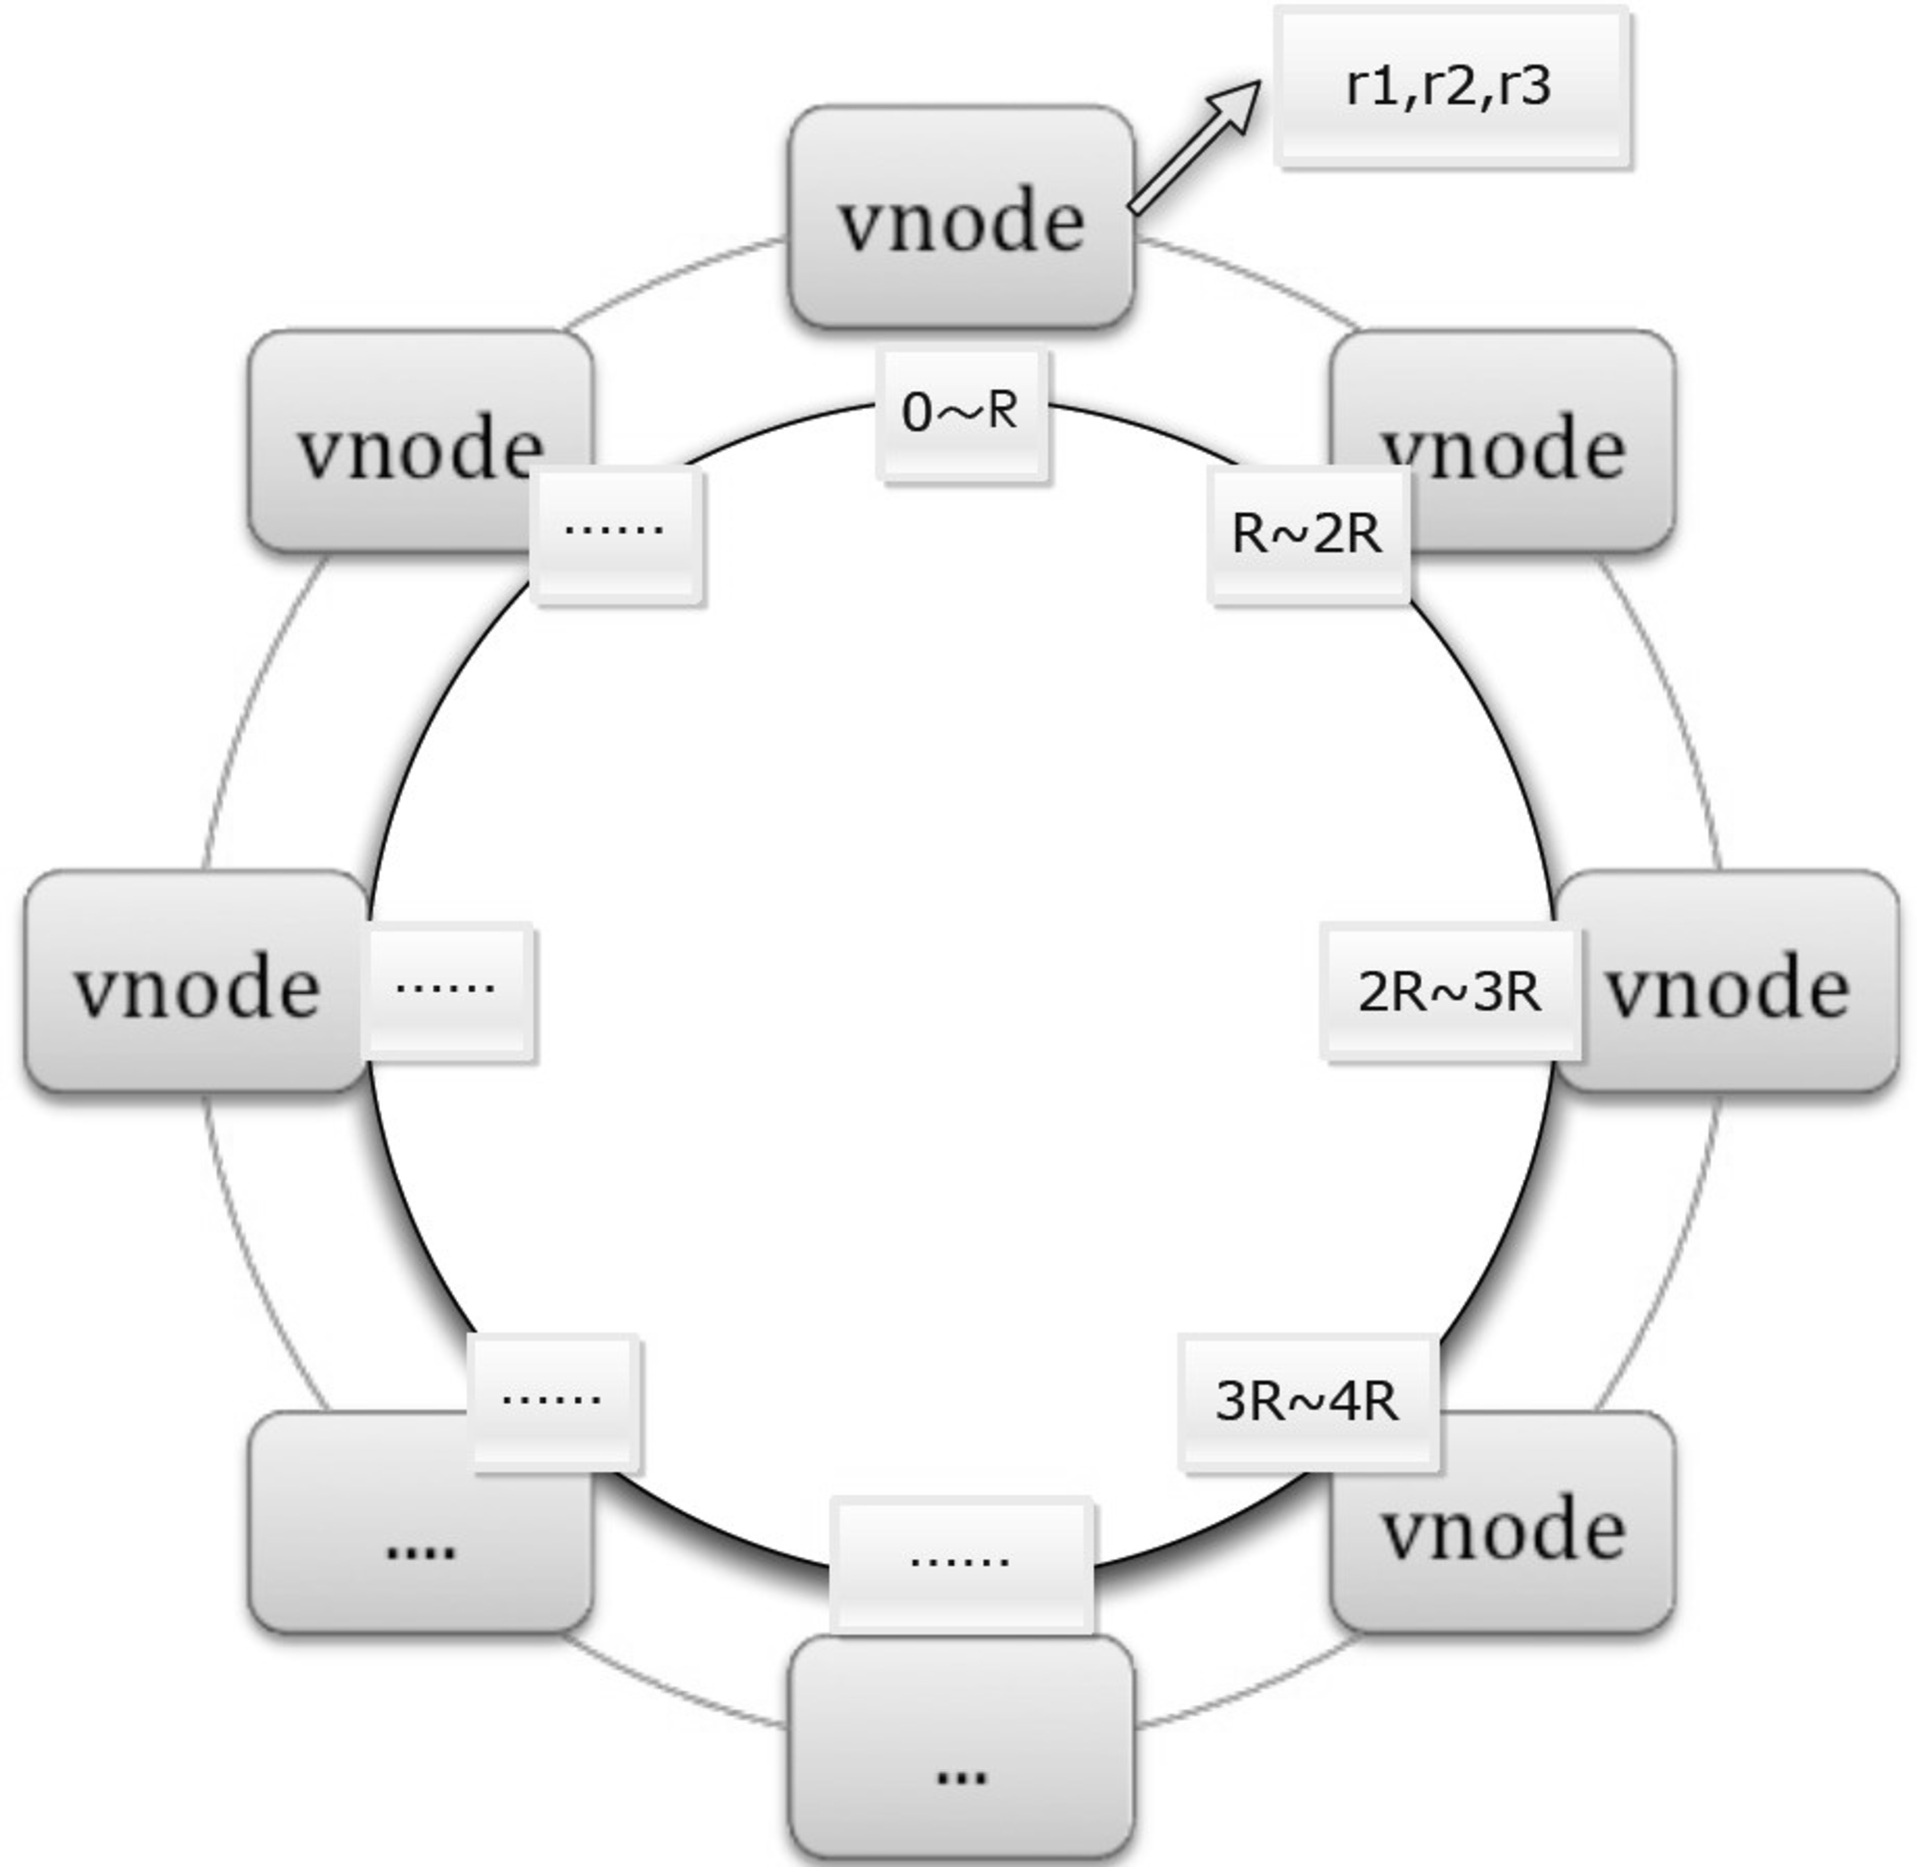
\includegraphics[height=3in]{../figures/vnode.pdf}
  \caption{Sedna虚节点环结构。其中存储着$0-R$的数据的虚节点被存储到实节点$r1$,$r2$和$r3$上}
  \label{fig:vnode}
\end{figure}

如之前所描述,基本的一致性哈希算法当面临节点不断加
入或者离开集群的时候,会导致节点之间存储的数据范围有很
大差别,从而使得集群性能不均衡,这对于构建基于有限内存的的存储集群来说问题更明显。Sedna中使用虚节点策略能够有效减少集群中数据的不均衡性:虚节点作为数据存储的最小连续块,其与访问相关的数据都会被记录下来,比如它当前存储的实际数据的容量、读写的频率等。这些信息被用来计算形成一个全局一致的实节点负载表。该负载表记录了所有存储这些虚节点的实际物理节点的负载情况。根据这个负载表,我们将数据以虚节点为单位进行数据迁移或者将新的虚节点存入负载较轻的实节点中。在Sedna中,该负载表存储与ZooKeeper子集群中,考虑到分布式读写的性能问题,均衡表不需要每次系统进行读写数据之后就更新,更新首先都是在每一个物理节点本地进行,所有的更新在本地经过计算和分析后,最终周期性的更新到负载表中。

Sedna的数据分割算法结合了一致性哈希算法和集中式的元数据管理。后者主要体现在Senda对虚节点到实节点映射信息的集中管理。Sedna中虚节点和实节点的对应关系并非像之前介绍的一致性哈希算法那样,通过在环上进行顺时针指定,该映射关系是动态可变的,可以动态改变意味着更简单的负载均衡策略,同时也意味着映射信息需要集中的存储和管理。在Sedna中,这些信息保存在图\ref{fig:sedna}所示的ZooKeeper Cluster中。这部分数据的存储和读取对系统性能影响很大,我们将在后面具体介绍它的设计和优化,并且通过实验证明该方案对系统性能的影响可控。

\subsection{数据备份}
数据备份是分布式存储系统中常用的提高数据可靠性的方法。通过将数据保存在多个服务器上,系统可以在部分节点失效的情况下继续提供数据读写服务。由于内存中的数据在掉电后无法重建,因此数据多节点备份在基于内存的分布式存储系统中更加重要。

Sedna系统中每一个数据都至少包括两个备份以保证数据的可靠性。多个备份之间由于节点崩溃,网络延迟等原因,存在不一致的可能,在Sedna中我们使用基于议会选举(quorum)的最终一致性来维护不同拷贝之间的一致性。

\begin{quotation}
假设分布式系统中,每一个节点有$N$个备份,并且假设当我们从这个$N$个备份中读取到超过$R$个一致的数据的时候,我们才认为读成功,并且返回给用户;当从$N$个备份中写入成功$W$个,才认为写成功返回。那么当$N,R,W$满足下面公式(\ref{equa:quorum})的时候,我们就可以保证每次成功读写都得到一致的结果。比如,如果每一个数据有三个备份(这也是通常情况下数据中心中备份的情况),设置$R=2$,$W=2$,此时公式\ref{equa:quorum}得到了满足,那么在这种情况下,如果一次写成功,那么就意味着至少有两个节点上已经写入了正确的结果,如果此时发出读请求,由于至少在两个节点上得到一致的结果才会返回,那么一旦返回的时候,我们可以确定返回的是刚刚写入的值。

\begin{equation}
  \label{equa:quorum}
  \begin{split}
  R + W > N  \\
  W > \frac{N}{2}
  \end{split}
\end{equation}

\end{quotation}

Sedna中的读写都是通过一个协调节点实现的,如图\ref{fig:sednareplicas}所示。来自客户端或者内部应用程序的请求通过路由器会被发送到Sedna机群中任意一台服务器,此时这台服务器就成为这次读写请求的协调者。协调者负责查询所需要的数据所在的物理节点所在的位置,并发的向存有这些数据的实节点发送请求,根据请求返回的数据的时间戳来判断是否有足够数目的一致结果。在得到足够数量的一致结果之后马上返回结果给调用者。使用协调节点能够有效的均衡客户端请求带来的压力,并且协调节点除了负责执行Quorum算法外,更重要的是还要负责起数据恢复和最终一致性的功能。

\begin{figure}[h!]
\centering
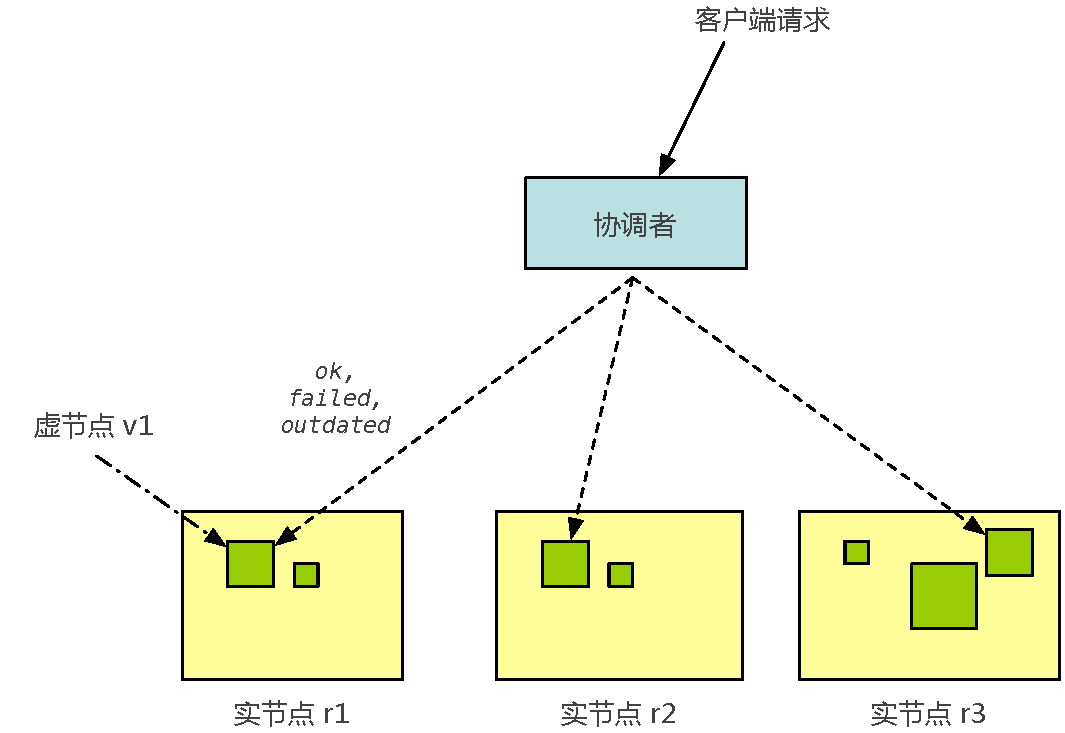
\includegraphics[width=5in]{../figures/sednareplicas.pdf}
\caption{Sedna使用协调者进行多备份读写过程}
\label{fig:sednareplicas}
\end{figure}

为了保证数据的可靠性,Sedna中每一个数据保持了多个备份。对一个集群来说,服务器离线重启再上线的情况会经常发生,因此系统中经常出现备份不足或者备份之间数据不一致的情况。Sedna并不强制要求每一次读写过程中所有的数据都一致,而是采用了最终一致的策略:对于那些数据不一致的节点,Sedna会启动异步的过程对其中数据进行强制同步,这个修复过程发生在\textit{数据读}的过程中,我们称为\textit{读恢复}。读恢复发生在协调节点上。当协调节点向多个备份发送读请求的时候,那些离线或者崩溃的节点会出现超时的情况(如图\ref{fig:sednareplicas}所示)。按照Quorum算法的要求,对于达到了公式\ref{equa:quorum}的读写请求,但仍有部分节点返回不一致的数据的情况,协调者在返回给客户端正确的请求数据之后会开始数据恢复工作。

对于超时或者拒绝服务的返回值,协调节点会再次向ZooKeeper集群确认该节点是否离线或仅仅是协调者本身出了问题。如果确认对方节点确实已经离线,协调节点会异步的启动一个数据备份任务,将数据从已存的物理节点中拷贝到新制定的节点中去,并且在拷贝完成之后修改数据的映射信息。

\subsection{节点管理}
节点管理主要包括:1)对集群中的现有节点的状态进行监控,及时发现节点失效的问题,并采取对应的措施;2)对新加入集群的节点进行管理,进行数据迁移,维持集群的负载均衡;3)对由于软硬件错误离开集群的节点进行管理,维护集群的稳定性。

Sedna对于节点加入和退出都是自动处理的。如果集群中新加服务器,只需要在其上启动Sedna实例即可。如流程图\ref{fig:sednastart}所示,每一个刚启动的Sedna实例都首先启动本地的内存管理模块,之后申请连接ZooKeeper Cluster来同步状态。如果ZooKeeper服务还没有初始化完成,这意味着整个Sedna集群还没有启动,该Sedna实例会申请一个全局锁,并初始化整个集群。对于ZooKeeper已经成功启动的情况,所有新加入的节点都会通过在ZooKeeper的$real\_nodes$目录下创建一个临时Znode节点($ephemeral$)来表明自己的存在;完成后,本地会启动一定数目的线程(根据及其性能来配置)来从当前负载较高的服务器上请求虚节点数据,并且存储到本地。当该动作完成后,它会改变集群中虚节点到物理节点的映射关系。因此它需要最后向ZooKeeper子集群申请修改这部分数据。在Sedna中,虚节点的数目是在集群启动前写入到配置参数中的,一旦集群启动后,不能够更改。节点在加入系统之后会启动一定数目的线程来从别的物理节点拉取数据,这个线程数目可以根据虚节点的数目进行调整。

\begin{figure}[h!]
\centering
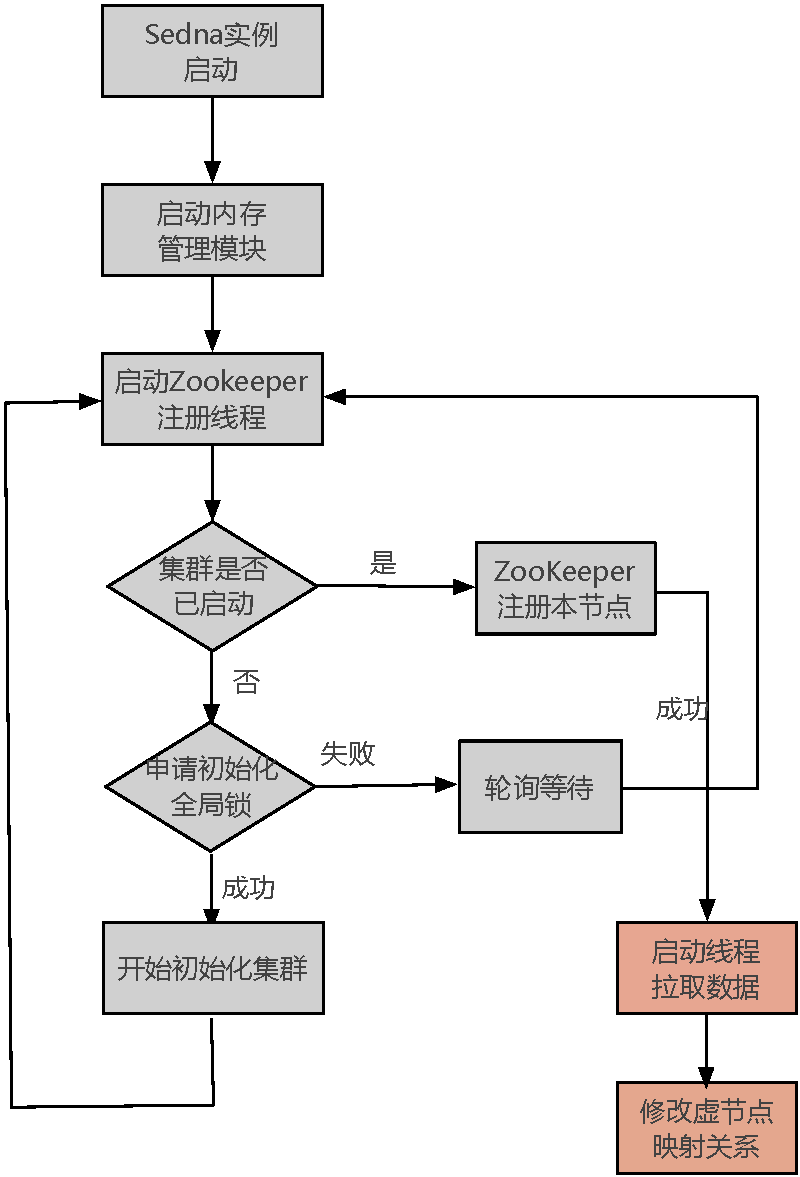
\includegraphics[height=4in]{../figures/sednastart.pdf}
\caption{Sedna中节点加入服务的流程图}
\label{fig:sednastart}
\end{figure}

当一个节点意外的离线或者崩溃的时候,之前维持的节点和ZooKeeper集群之间的心跳信息丢失。这个动作会提醒ZooKeeper有节点离线了。此时Sedna集群并不会立即做出反应,节点丢失的恢复工作主要由读操作的时候指派的协调者来执行。

\subsection{ZooKeeper子机群}
Sedna使用Zookeeper\cite{hunt2010zookeeper}子集群来实现分布式锁及元数据管理。Apache Zookeeper是一个开源的用于开发大规模分布式程序中分布式协调的组件。它是一个中心化的服务,可以用来存放全局一致的配置信息、名字空间信息、提供分布式的同步或者组服务。ZooKeeper是基于ZAB(ZooKeeper Atomic Broadcaset)\cite{junqueira2011zab}协议的,ZAB是一种类似Paxos的分布式一致性协议,其性能好于现有的Paxos\cite{lamport2001paxos, lamport2006fast}实现。

ZooKeeper服务会在Sedna集群的一部分节点上运行,这部分节点就构成了图\ref{fig:sedna}中的ZooKeeper Cluster。该子集群中节点的数目可以根据Sedna集群规模变化而变化。ZooKeeper Cluster在Sedna中的作用非常重要,本节中我们将分析Sedna中ZooKeeper的使用,并且针对性的设计优化的策略。

图\ref{fig:zkper}展示了ZooKeeper版本3.2运行在拥有双核2Ghz的Xeon以及双SATA磁盘上的性能图。读请求共1K个,写请求也为1K,服务器(Servers)表明了Zookeeper所管理的服务器数目,除了这些ZooKeeper服务器外,试验中采用了超过30个额外的的服务器模拟客户端请求。

\begin{figure}[h!]
  \centering
  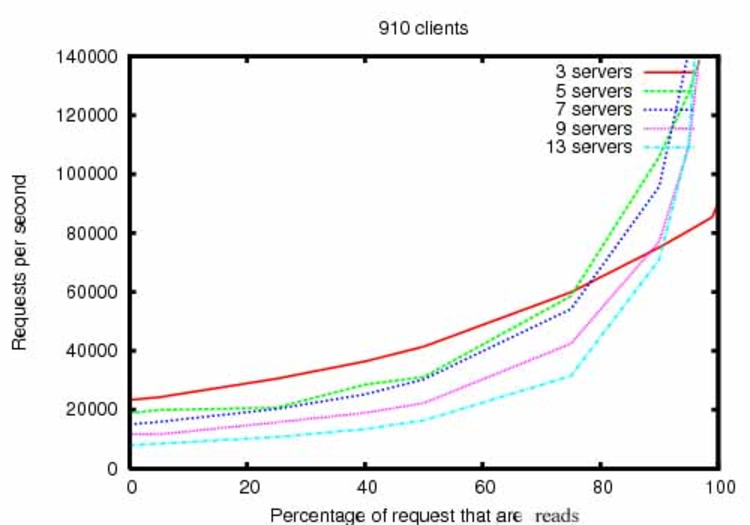
\includegraphics[width=3.5in]{../figures/zkp.pdf}
  \caption{ZooKeeper性能随着读写比率变化图}
  \label{fig:zkper}
\end{figure}

通过上述试验我们给出ZooKeeper的性能特点总结:

\begin{enumerate}
\item 请求中读占的比重越大,ZooKeeper集群能够响应的请求数目越多。
\item 对于读请求,ZooKeeper的性能随着服务器数目的增加而提升;对于写请求,性能反而会随着服务器数目的增加而降低。
\end{enumerate}

这两点很容易理解,因为客户端读数据的时候仅仅需要连接ZooKeeper集群中任意一台服务器即可。但是写请求需要传播到ZooKeeper集群中的多台机器,从而使得效率较低。根据上面优缺点可见ZooKeeper本身是一个写效率较低而读效率较高的系统,因此在Sedna中对ZooKeeper将尽量使用读而不是写,需要写的主要有两种情况:

\begin{enumerate}
  \item 当Sedna集群首次启动的时候,所有的物理节点都需要向ZooKeeper创建代表自己的\textit{znode}。除此之外,负责初始化的节点首先还需要单独向ZooKeeper写入代表所有虚节点的\textit{znode}。典型的Sedna配置中可能包括数百万条虚节点,因此这些动作会产生大量的写操作。
  
  \item 当物理节点加入或者离开集群的时候,Sedna会自动更新系统中表示物理节点的znode的数据。当我们因为数据均衡或者数据一致性需要对数据进行迁移的时候,需要修改虚节点和物理节点之间的对应关系,这是通过写ZooKeeper中数据实现的。
\end{enumerate}

前一种情况虽然非常耗时,但是由于其只会在集群启动的时候执行一次,因此我们不会将其作为性能瓶颈来考虑。后一种情况在系统运行时会时有发生,但是以ZooKeeper毫秒级的写速度,这种情况即便发生也不会对Sedna的性能产生明显的影响,这在实验中也得到了验证。

ZooKeeper的读性能是Sedna的另一个性能瓶颈。为了避免这个瓶颈,我们使用了如下三个策略:1)大量使用本地缓存。Sedna中协调者进行读写操作的时候优先从本地缓存中获取数据,当缓存数据被证明失效的时候才会从ZooKeeper中更新新的数据。2)为了减少由于缓存失效带来的长时间延迟,我们在每一个Sedna实例中还会启动一个周期线程负责从ZooKeeper中更新数据的映射信息。该线程执行的周期称为\textit{租约时间}。租约时间是不断变化的:当最近对于ZooKeeper中的数据有写入,那么租约时间就会减半;如果在上一个租约时间内ZooKeeper中没有数据改变,那么下次租约时间就会延长一半。3)每次对ZooKeeper中数据进行更新的时候,系统会将其记录在单独的\textit{znode}目录下,这样无论在写入和读出的时候都能够避免锁,其次在ZooKeeper中我们关闭监控(watch)功能以防止因为大量的节点监控同一个znode节点,导致的该节点上任何一个改变引发大量线程突然启动的惊鸿效应。

\subsection{基本数据访问API}
\subsubsection{写操作}
由于在web2.0应用中,随机写是一种非常普遍的操作,Sedna存储系统允许来自不同客户端对相同的键进行无锁并发写操作。Sedna中所有的键值对数据都有时间戳的保护,并且每一个键所对应的值都不是单一的一个值,而是一个列表,列表中保存了来自不同的协调者所写入的最新的值以及当时的时间戳,列表的第一个元素则维护着来自不同的协调者写入的所有数据中时间戳最新的那个值。Sedna为写操作提供了两个不同的API:\textbf{write\_latest()}和\textbf{write\_all()},他们两个都是无锁写。

用户调用\textbf{write\_lastest()}函数时,Sedna会将请求的时间戳和当前该数据最新的时间戳进行比较,对于试图以较旧的时间戳更新当前较新的数据的请求会返回一个$outdated$,而那些具有更新时间戳的写请求将直接覆盖当前数据,并且返回给用户$ok$。而如果用户调用\textbf{write\_all()},那么Sedna只会将请求的时间戳与该数据上次来自相同协调者所写的版本号做比较。如果当前请求比较新的话则会更新那个来自,否则返回$outdated$。

任何程序调用写API都会得到三个不同的返回值(如图\ref{fig:sednareplicas}所示):$ok$代表当前数据被成功写入并且覆盖原有数据;$outdated$表示当前数据比较老,未能覆盖掉原有数据;$failure$表示由于网络等原因写失败。

\subsubsection{读操作}
键值存储系统的读API都非常简单,给定一个键,返回当前键对应的数据。由于Sedna中所有的值都根据它们来源和时间戳进行管理,我们也对应提供了\textbf{read\_latest()}和\textbf{read\_all()}两个API给应用程序快速的获取值。如字面意思所示,\textbf{read\_latest()}会返回最新的数据,不管当前读操作所在的协调者是什么状态;而\textbf{read\_all()}则会返回当前键对应的来自不同协调者写操作的所有数据,这些数据被维护成一个列表发送给客户端。如何处理这些数据的不一致将是客户端软件的工作。

\subsection{持久化策略}

Sedna实现了两种不同的持久化策略:周期刷新和写前日志。写前日志不是默认的持久化方式,它只是对于特定的应用可以启动,用来应对非常严格的数据持久化要求,而周期刷新作为日常情况下数据的持久化策略,已经足够保证Sedna中数据的高可用性。

我们首先分析一下周期刷新策略的可用性。在一个有$n$个服务器的集群中,假设所有的节点都有相同的MTBF\cite{mtbf}值为$m$,那么每一个服务器在时间间隔$t$内发生失败的概率为$\frac{t}{m}$。如果当前Sedna集群中共有$v$个虚节点,那么从某一个虚节点中读取数据的概率为:$\frac{1}{v}$。假设周期刷新的周期为$T_{f}$,以及整个Sedna集群
的读写的带宽为$tp/s$.

Sedna出现丢失数据的条件是比较苛刻的,它要求:1)一个数据的三个备份都在短时间内发生故障;2)其次这个时间段内没有发生过任何数据刷新到磁盘的动作;3)并且这个时间段内也没有任何来自客户端的对该失效节点上任何一个虚节点进行访问。那么发生这三个事件的概率是可以计算的:

\begin{displaymath}
P_{f} = (1 - \frac{1}{v})^{tp* T_{f}}(\sum_{i=3}^{n}  (\frac{T_{f}}{m})^{i} (1- \frac{T_{f}}{m})^{n-i} ( 1 - \frac{C_{v}^{ik} C_{ik}^{k}\cdots C_{2k}^{k}}{(C_{v}^{k})^{i}}))
\end{displaymath}

根据上面的公式所示,$P_{f}$是一个非常小的数。假设一台服务器的
$m=50,000$小时,$n=1,000$,并且$T_{f}=600$,那么$P_{f}$小于
$2e^{-20}$. 因此我们认为在Sedna中使用三个备份,并且周期性的将数据刷新到磁盘中的方案在统计意义上来说是足够保持数据的可靠性的。


\subsection{Sedna实时数据访问接口}

Sedna是为实时应用设计的分布式存储系统,除了将数据完全放入内存中来提高系统的读写速度外,设计了新型的基于层次的存储架构来提高系统的扩放性外,更重要的是Senda实现了一套实时数据访问接口帮助用户编写复杂的实时应用。

为了支持用户多种多样的实时应用的需求,Sedna增加了基于触发的API作为其基础功能。触发适合实时处理的关键在于,它对于数据的更新极为敏感。每当数据发生变化的时候,触发快速执行需要的动作,能够很快的给出用户需要的结果。触发机制在数据库中作为辅助工具已经广泛使用多年,这些功能在数据库中往往是作为确保数据完整性、合法性检查而出现的,不过我们在Sedna中设计的触发API和数据库中的触发器还有所不同,主要差别体现在Sedna运行在大规模的分布式集群中,其面临着更加复杂的调度和管理任务:不断执行的多个触发之间如果有相关性的话如何在存储层进行控制,如何帮助上层应用进行负载均衡等。

一个基于Sedna的触发API实现的典型的实时应用程序通常包含了若干个对数据的触发访问来完成计算任务。如图\ref{fig:triggers}所示,我们用三个触发器A、B、C来构成一个计算任务。触发器A会监测初始数据集的并且产生中间结果写入Sedna系统中,这些中间结果的改变会触发触发器C执行,C执行的结果会导致触发器B执行,而B最终将再次触使A执行。以此往复。A、B、C共同构成了一个循环任务的三个子部分。

\begin{figure}[h!]
  \begin{center}
    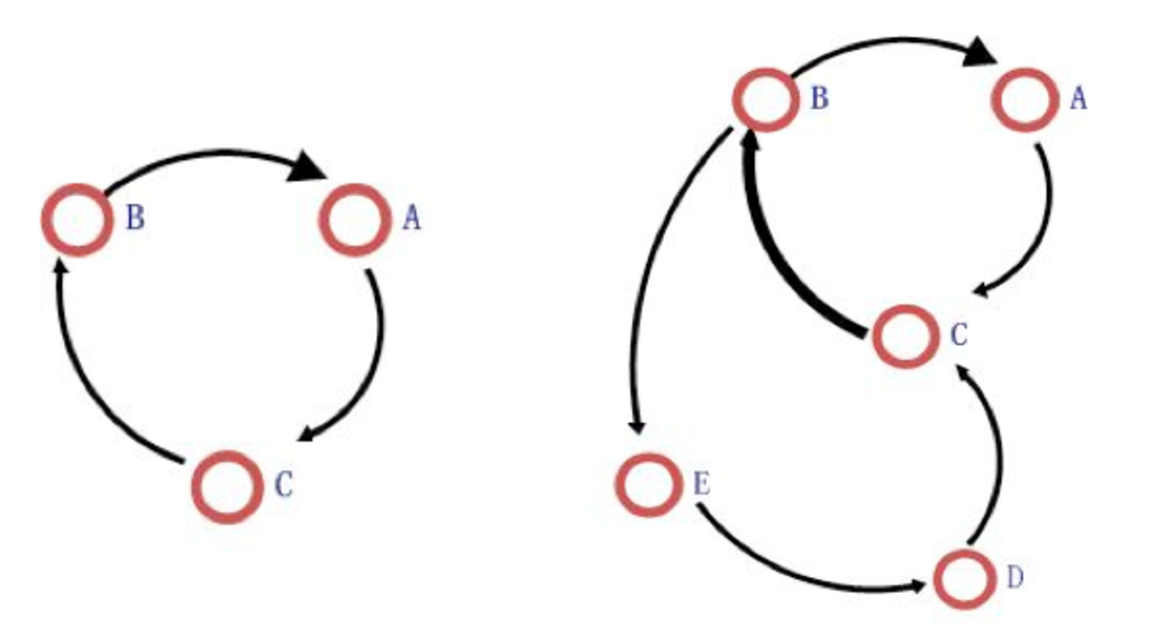
\includegraphics[width=4in]{../figures/domino.pdf}
    \caption{Domino提供的基于触发的实时数据访问接口的典型应用实例}
    \label{fig:triggers}
  \end{center}
\end{figure}

\subsubsection{流控制}
Sedna中基于触发的API简单易懂,然而在一个分布式存储中广泛的提供这种API却面临着种种问题,其中最重要的挑战在于如何解决由多个触发API调用带来的可能的涟漪问题。我们依然使用图\ref{fig:triggers}来描述这个问题。图\ref{fig:triggers}中右图展示了Sedna之上的应用调用了A-E共5个API,我们称应用使用了5个触发器A-E。执行过程中,A、D两个触发后执行的结果一步激活了触发器C,而C的执行结果反过来又导致A和D的执行,由触发器相互激活形成的环可以用来支撑一些复杂的应用,然而在本例中,一旦循环开始,每一轮下来所有触发器被激活的概率都会提高一倍并且最终将整个集群的资源占完。并且由于Sedna是作为一个存储系统存在的,多个独立的用户会共同使用同一个集群,由于互相之间并不了解对方的应用,因此出现这种情况的概率就更高了。我们通过在Sedna的触发API中引入token机制来平衡触发执行的速率。每一个触发器的执行都需要一定的周期来获得token,对于那些在没有获得token的时候数据更新,API将会自动忽略,并且不会返回数据给用户程序。下面的代码展示了如何利用Sedna的实时API编写一个简单的应用(基于Java)。由于Java不是函数语言,所以开发者需要将执行的动作封装成一个简单的Java类,并且提交给Sedna实时API。对于Sedna的实时API来说,每次调用都需要指定API所监控的键或者键的范围,数据发生改变时需要接管的类。每一个传给实时API的类都必须是Action类的子类,其中关键的action函数将获得新写入的数据的值,并且负责进行处理。

\subsubsection{Sedna实时API应用的示意}
\begin{lstlisting}[language=java]

public class myAction extends Action<Key, Iterator<Value>, Result>{

  protected void action(Key k, Iterator<Value> vs, Result){
    //user codes here
  }

  protected boolean filter(){
    //user codes here
  }

  public static void main(String[] args){
    SednaClient instance = new SednaClient();
    instance.ReadTrigger(KeySet, myAction.class);
  }
}
\end{lstlisting}

在上面例子中,首先我们实现了一个Action的子类myAction来负责执行用户逻辑,并且在主函数中调用SednaClient的实时触发API($ReadTrigger$),其中指定了需要处理的键的范围以及执行的动作类。在示例中还有一个filter函数,该函数也是Action基类中的函数之一,用户应该继承它来根据自己的需求设置停止条件。Filter机制基本包括两个方面:其一,filter函数是基于每一个键值对来调用的,Sedna运行时系统会根据filter函数是否返回true来决定是否执行用户动作;第二是filter函数使用的参数中包括了当前改变的数据以及改变前的数据,这样设计使得很多迭代收敛的任务能够更容易的基于Sedna实现。

\section{实验和性能分析}
\label{section:exp3}

本节中我们将对Sedna存储系统的性能进行实验分析。在Sedna中,我们使用了修改版本的Memcached作为本地内存存储,因此它的性能受到Memcached性能的限制。然而通过跟Memcached的性能比较我们可以看出,即便作为一个分布式的存储系统,Sedna依然具有和Memcached可比的性能特征,并且能够提供Memcached这类缓存系统所不具备的持久性、扩放性等特征。在试验中,我们并没有将Sedna和别的基于内存的键值数据库来比较,比如MemBase\cite{membase},主要原因是这些系统的并非基于Sedna所依赖的Memcached实现的,并且设计的主要目标也不同,使得这种比较不够公平。我们相信,通过和广泛应用与业界的Memcached性能进行比较,我们能为Sedna系统的性能设定一个标准的比较值。别的系统通过和Memcached性能进行比较就可以相比较出和Sedna的性能差别。

本节所有试验都基于一个有9台物理服务器的实验集群,其中每一台服务器都
使用Xeon双核2.53Ghz处理器以及6GB的内存。所有的物理机器都通过一个GB的以
太网互联,节点之间没有划分机架,所有节点之间的消息传递的时间在毫秒以内。
所有Sedna实例服务器分为两种,一种单纯运行数据存储功能,我们为每一台节
点预先开辟4GB内存作为本地数据存储;另外一种节点构成了ZooKeeper子集群,
因此其上还需要运行Zookeeper服务,我们为每一台节点开辟3GB内存存储本地数
据。同时我们还使用Memcached在相同的实验集群上配置了相同的内存容量来进
行比较

\subsection{单客户端性能}

在本测试中,系统中只有一个客户端分别对Sedna集群和Memcached集群来进行
读写请求。所有要存储的键值都非常小,因为数据的大小并不是影响Sedna系统
性能的核心因素,数据大小仅仅会对网络带宽有影响。为了让所有的测试可比较,
我们每次都随机产生一个20字节的键,比如$test-000000000000000$,以及一个
20字节大小的固定值写入Sedna中。

\begin{figure}[h!]
  \centering
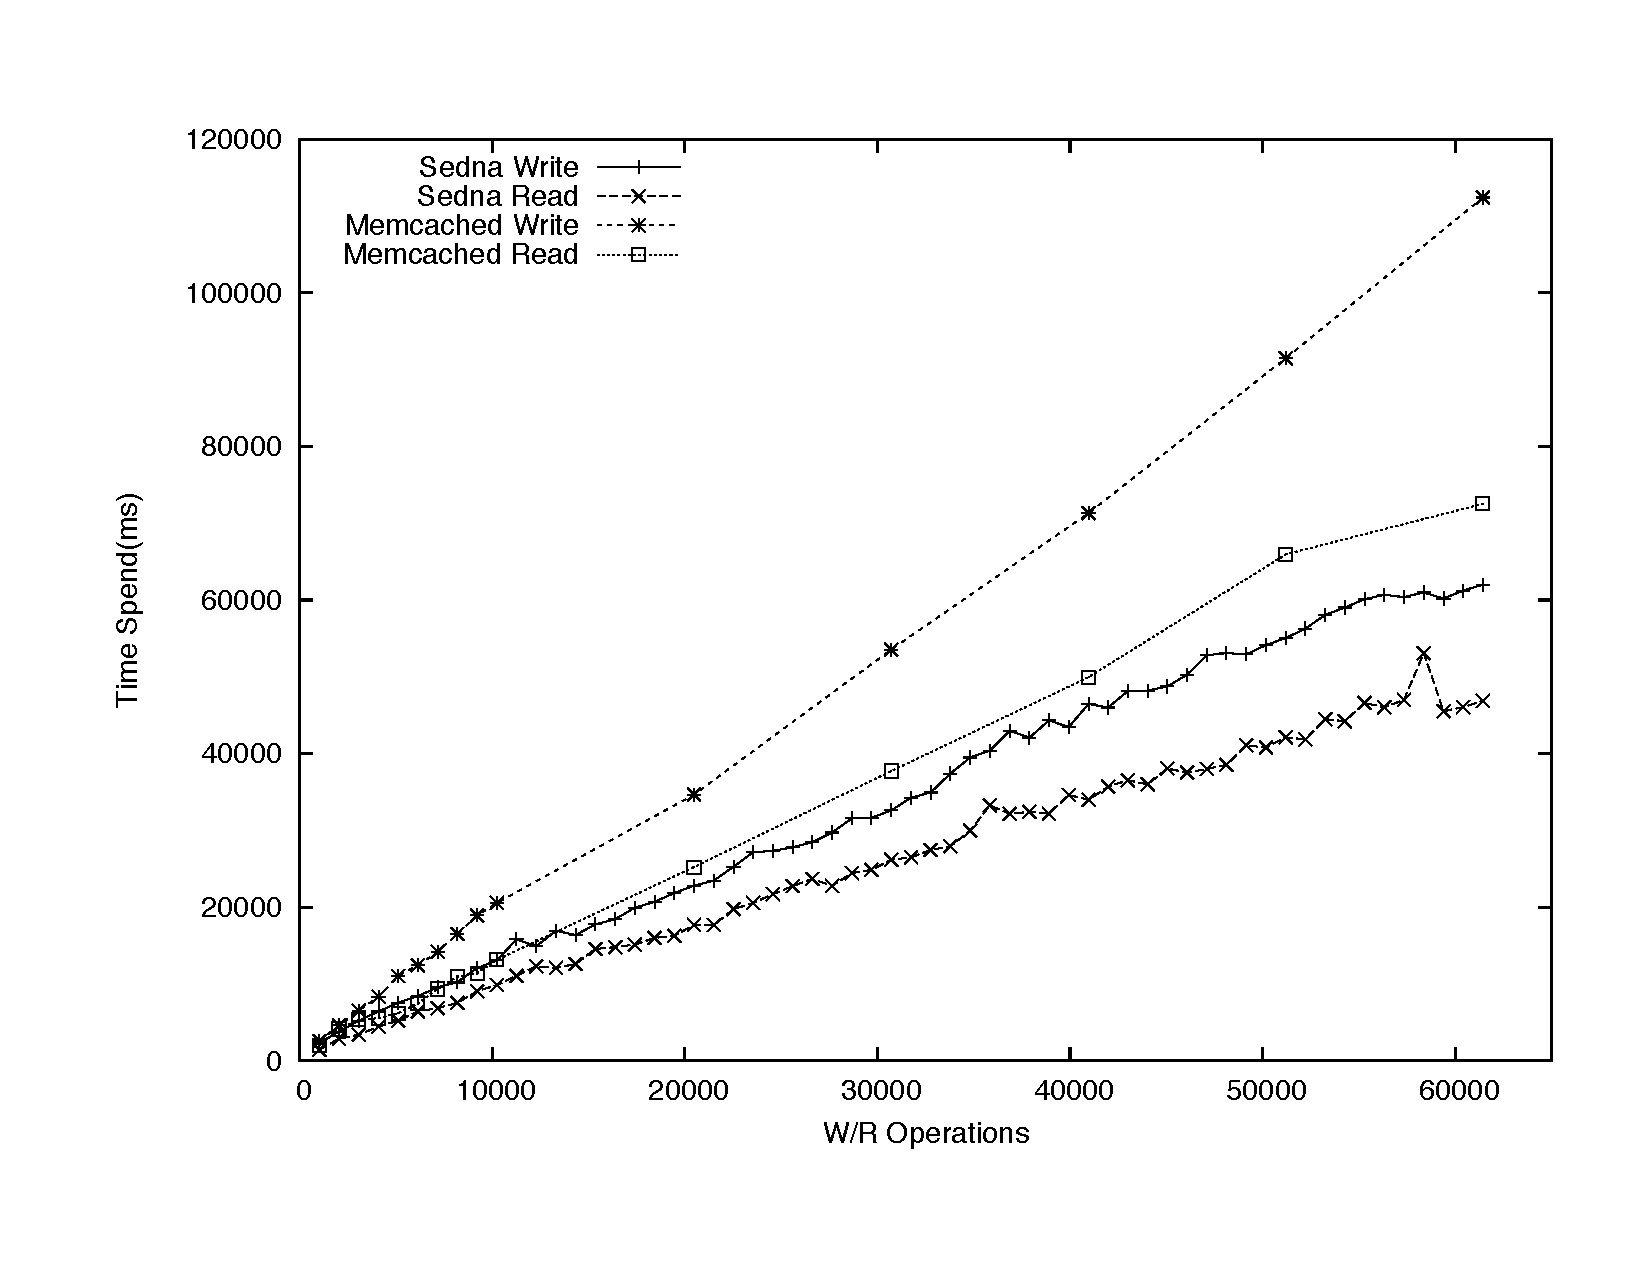
\includegraphics[width=5in]{../figures/compare_one_client_memcached_three.pdf}
\caption{Memcached客户端向不同的节点读写三次数据和Sedna正常读写的性能
  对比}
\label{fig:cp1}
\end{figure}


前面我们也描述了,为了给出比较标准的对比性能,方便与其他存储系统做比较,
所有的试验都以Memcached作为标杆。运行分布式的Memcached集群不需要在服务
器端做任何的配置,很多Memcached的客户端本身就支持以一致性哈希的方法将
数据分割到不同的节点上去。当然了,Sedna本身作为一个支持持久存储的内存
存储系统,它和Memcached这样的缓冲系统还是有一个非常重要且会影响性能的
区别的:Sedna会将一个数据并发的向不同节点写入至少3处,并且在其中2处返
回成功的时候返回。而Memcached只需要写入一份数据即可。为了使得这两个系
统的比较更加清晰,我们先后强制要求Memcached的客户端读写三次数据和读写一次
数据与Sedna读写请求做一次对比,最终的结果如图\ref{fig:cp1}和
\ref{fig:cp2}所示。

\begin{figure}[h!]
  \centering
  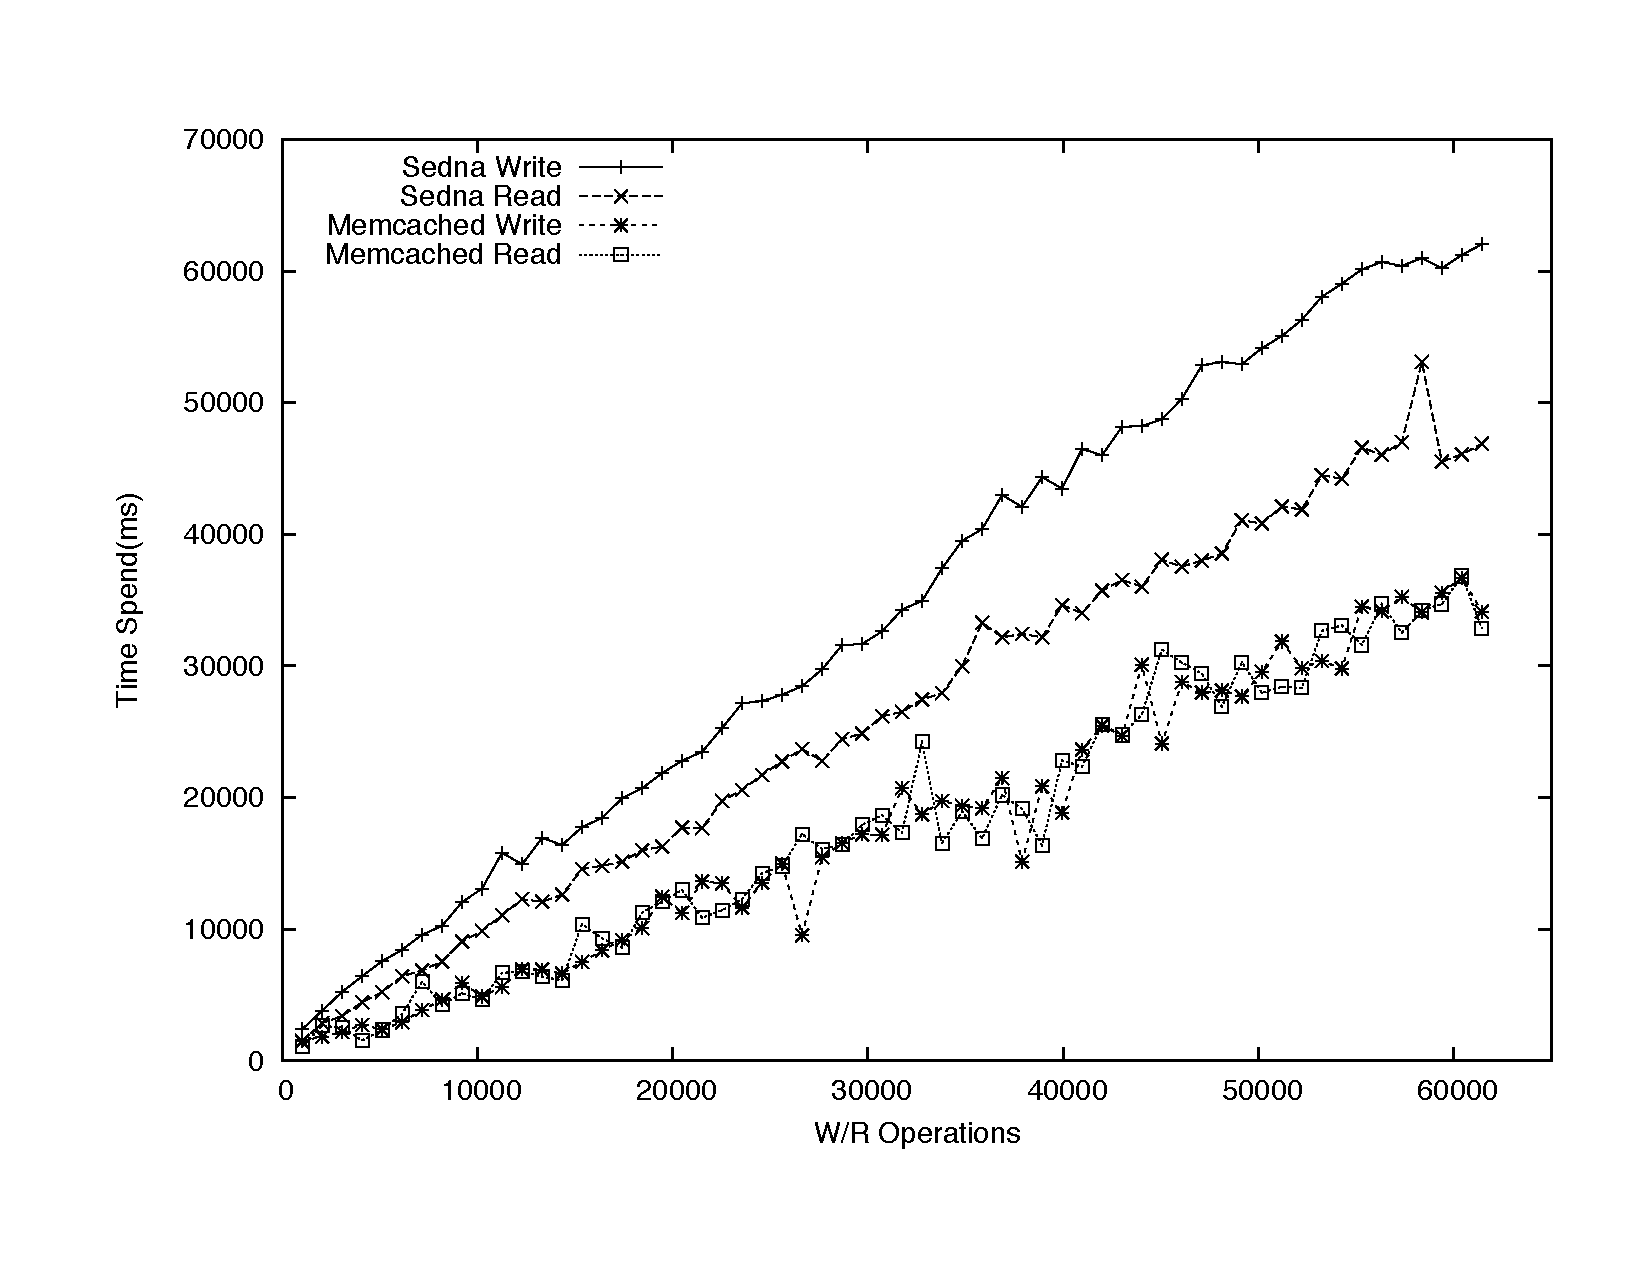
\includegraphics[width=5in]{../figures/compare_one_client_memcached_one.pdf}
  \caption{Memcached客户端向不同的节点读写一次数据和Sedna正常读写的性能
    对比}
\label{fig:cp2}
\end{figure}

尽管从图\ref{fig:cp1}中显示Sedna的读写性能都优于Memcached,实际上这里
面有一些不公平的地方:Memcached的三次读写是顺序进行的,而在Sedna中,我
们使用并发读写,并且使用了Quorum算法使得不需要等待最慢的读写完成,因此
性能要优于Memcached。之所以没有为Memcached设置并发读写,原因主要是如果
用户需要使用多次写入不同节点来保证数据的安全性,在客户端往往是通过依次
写成功来保证的。除此之外我们还在\ref{fig:cp2}中比较了Memcached只读写一
次的性能和Sedna的对比,可以看出来Sedna的性能比较稳定,一直保持高速的读
写能力,并且其速度比单纯memcached缓存系统稍慢,却明显快于在memcached中
用client实现多备份的做法。

\subsection{多客户端性能}

作为一个云计算平台下的分布式存储系统,通常不只一个客户端在进行读写请求,
系统中可能同时存在大量的应用从不同的节点请求读写。本节中,我们将在
每一个服务器上启动一个客户端同时发起读写请求。在这种情况下,网络带宽有
可能成为系统的性能瓶颈,在我们的试验中,所有的服务器都通过1GB以太网互
联。

图\ref{fig:perf}展示了9个客户端同时请求时Sedna的性能,图中的读写次数是
所有客户端读写速率的平均值。我们可以看出随着客户端数目的增加,每一个节
点的IO性能都有所下降。这很容易理解,因为多客户端导致的服务器负载增加,
网络带宽拥塞等。考虑同时有9个客户端在进行读写请求,Sedna系统整体的读写
带宽是远远超过单客户端的。通过这个试验我们也可以看出,Sedna在客户端数
目增加的时候,由于引入了协调者的概念,从而具备了很好的扩放行。

\begin{figure}[h!]
\centering
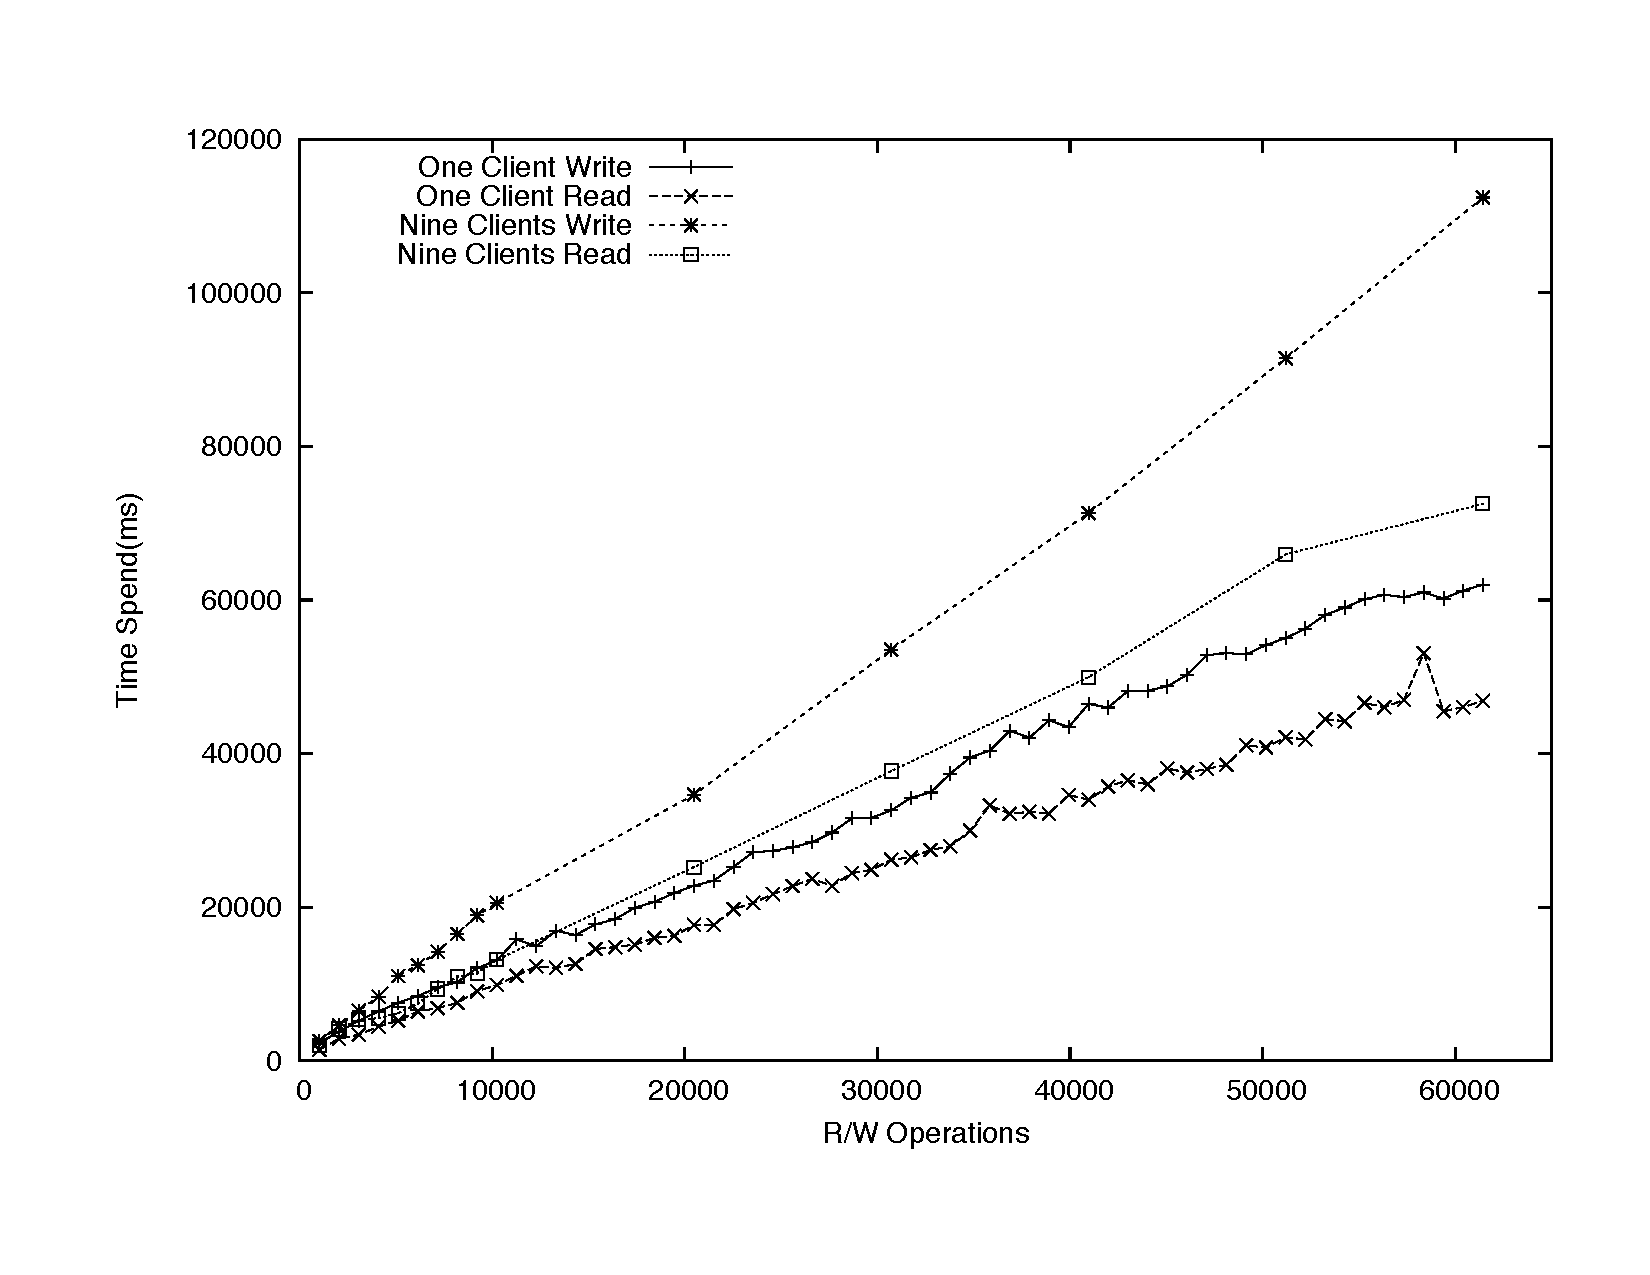
\includegraphics[width=5in]{../figures/sedna_one_client_nine_clients_compare.pdf}
\caption{多客户端和单客户端的读写性能对比(多客户端数据来自所有客户端的
  性能平均)}
\label{fig:perf}
\end{figure}

\subsection{ZooKeeper性能分析}

首先我们对本试验集群中运行的ZooKeeper集群进行一系列性能测试。从图
\ref{fig:zklatency}中可以看出一个同步的写操作在我们的集群中耗费了大约
10ms的时间,并且这个时间随着ZooKeeper节点的增加有所增加但是并不明显。
图\ref{fig:zkrlatency}展示了当ZooKeeper集群中节点数目增加时读延迟的变
化,我们可以看出当ZooKeeper读性能远远好于写性能。

\begin{figure}[h!]
\centering
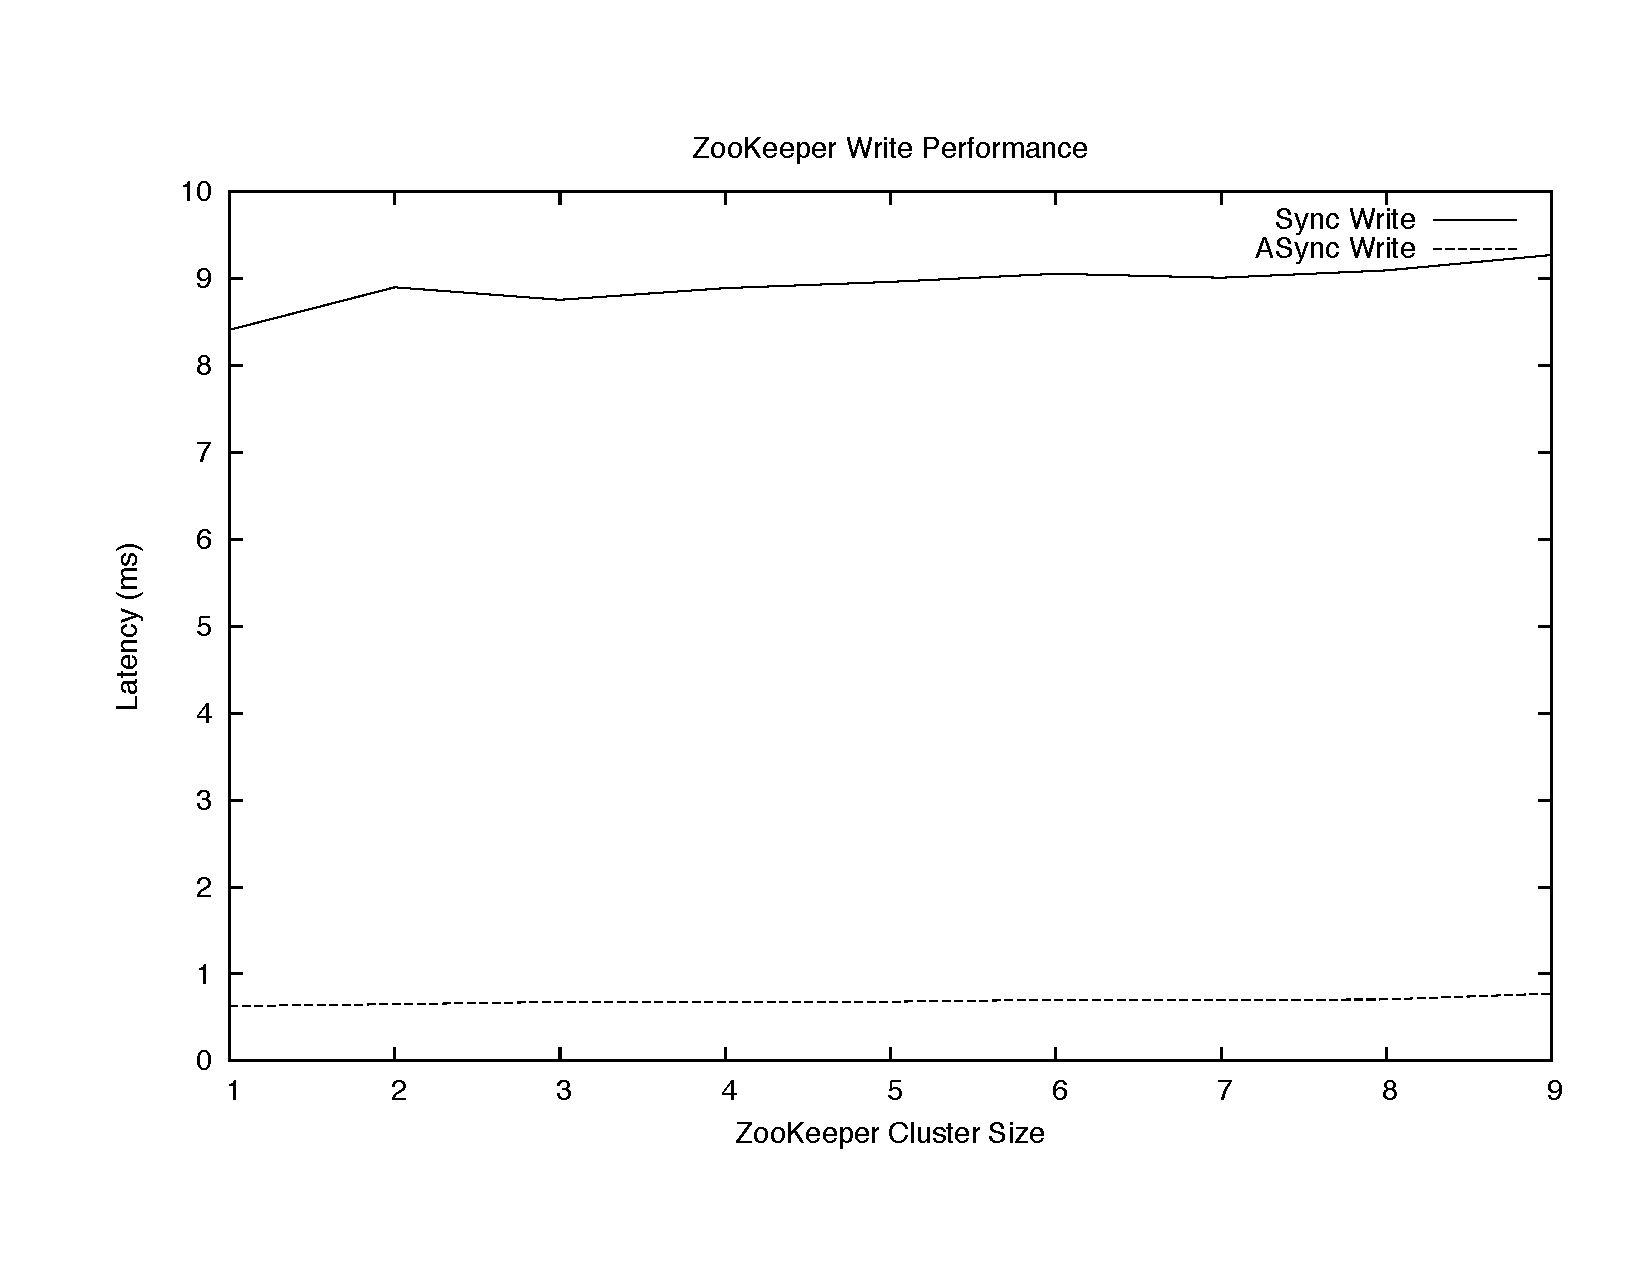
\includegraphics[width=4.5in]{../figures/zklatency.pdf}
\caption{ZooKeeper写延迟随着服务器数目的变化图}
\label{fig:zklatency}
\end{figure}

\begin{figure}[h!]
\centering
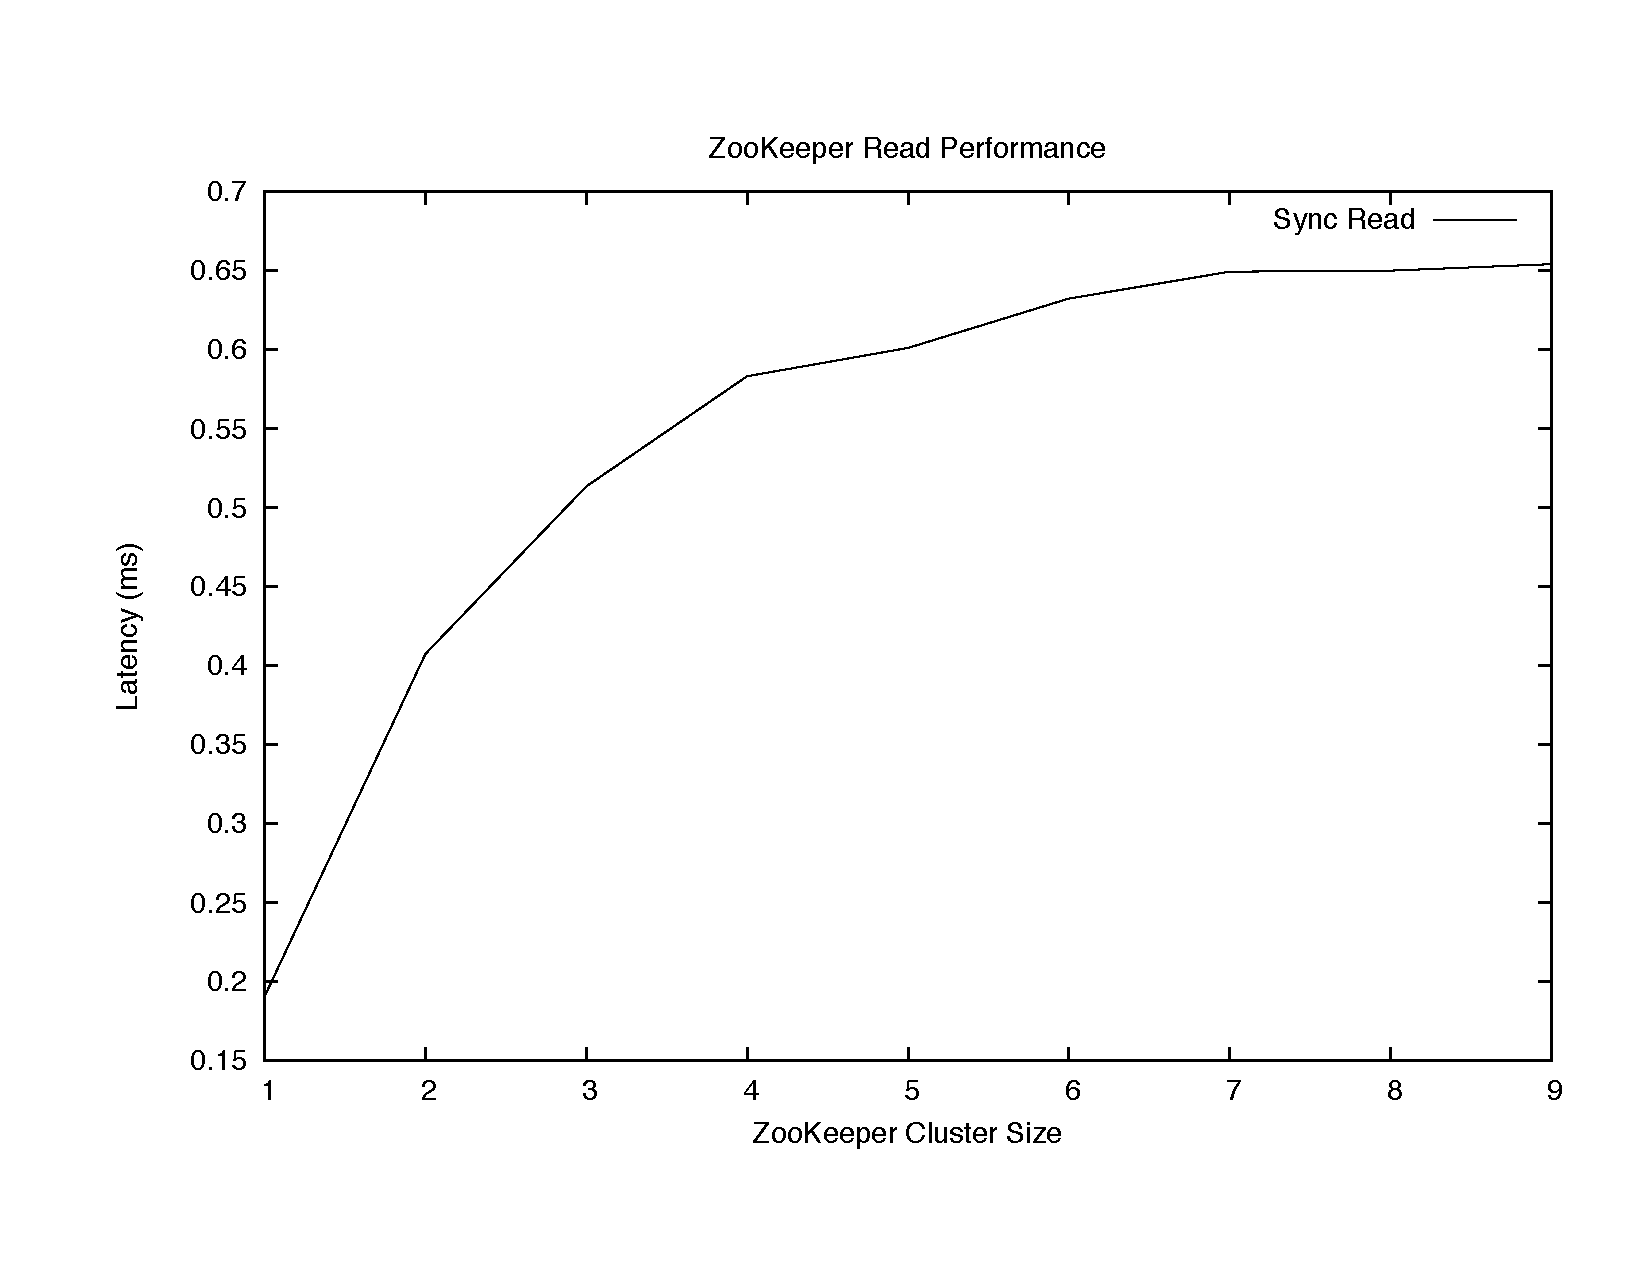
\includegraphics[width=4.5in]{../figures/zkrlatency.pdf}
\caption{ZooKeeper读延迟随着服务器数目的变化图}
\label{fig:zkrlatency}
\end{figure}

\begin{figure}[h!]
  \centering
  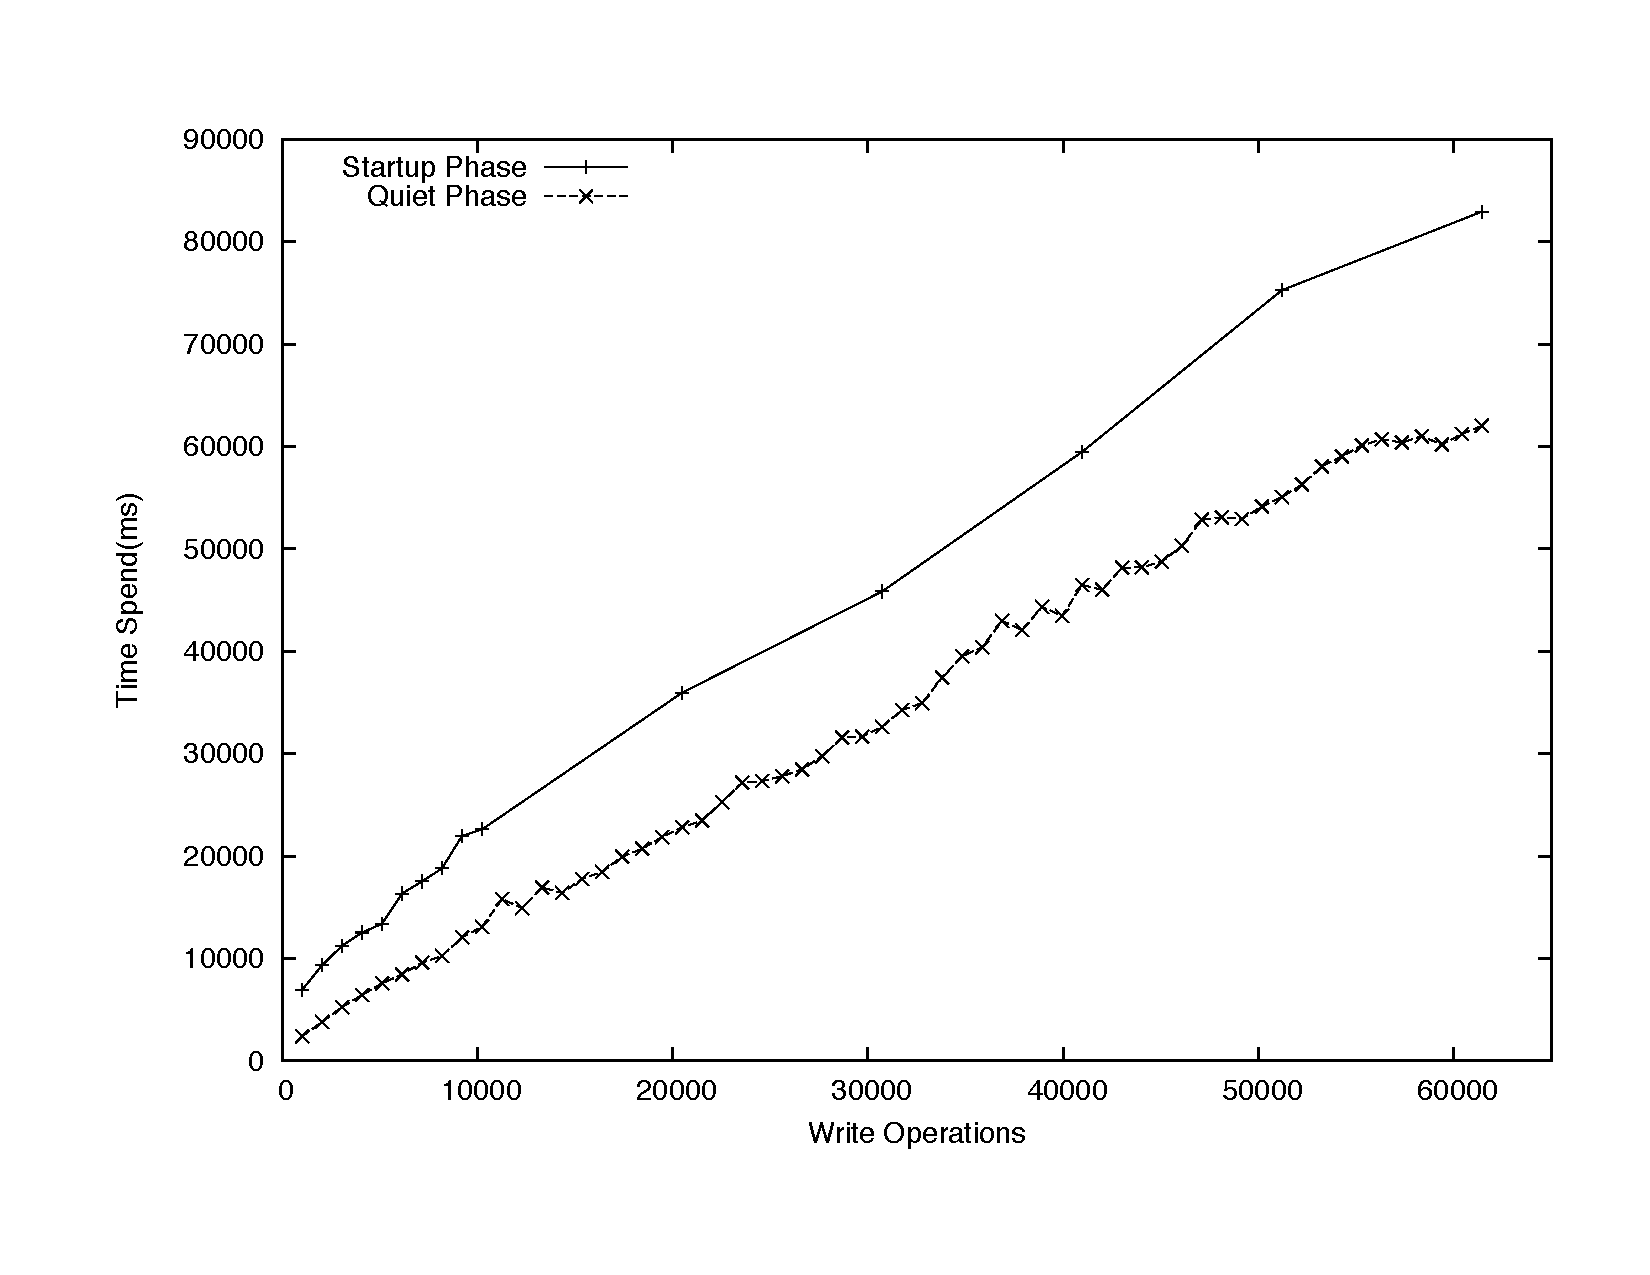
\includegraphics[width=4.5in]{../figures/sedna_write_quiet_startup_compare_one_client.pdf}
  \caption{启动模式和安静模式下单客户端性能对比图}
  \label{fig:zkquiet}
\end{figure}


为了证实ZooKeeper到底对Sedna系统性能的影响,我们在本实验中通过对启动阶
段性能和正常阶段的性能来比较。当Sedna集群第一次启动的时候,我们称这个
阶段为\textit{启动模式}。这个模式下,大部分的虚节点还没有指派给任何一个实节点,
此阶段需要进行虚节点的指派,需要非常频繁的写ZooKeeper。而这些写操作又
必须是顺序的,并且使得所有节点的本地缓存无效。这些动作会极大的降低
Sedna系统的性能。启动模式完成后,Sedna进入\textit{安静模型},在这个模式下,大
部分的虚节点都有了存储位置且相对稳定,且节点的缓存都是有效的,此时读写
性能达到峰值。通过观察这两个阶段的性能差别,我们可以看出最坏情况下,
ZooKeeper是如何影响Sedna系统性能的。从图\ref{fig:zkquiet}中可以看出,
这两个阶段的性能有一个比较明显的区别,不过两条曲线基本上保持了一个比例关系。

\section{小结}
\label{section:con3}
分布式存储系统作为云计算基础软件架构的核心对系统的性能起着至关重要的作用,为了支撑实时的云计算应用,我们设计并实现了一种完全基于内存的持久存储系统Sedna。Sedna能够在保证数据的持久性的前提下,为用户提供接近传统的内存缓存的性能。通过层次化的架构模型使得Sedna能够部署更多的服务器以提供与传统存储模型相同的存储容量。通过提供实时的API,我们进一步丰富了Sedna对实时应用的支持。通过对实时应用下存储系统的研究,我们认为使用内存作为优化只是解决了问题的一部分(提供了更快的数据的访问速度),而实际上我们面对的实时应用需要对数据的更新进行快速的反应,能够处理复杂的应用类型,这就需要计算模型的配合。因此,我们通过设计和实现一种基于触发器的通用编程模型来解决这个问题。
